\documentclass{book}\usepackage{knitr}

% Preamble

%%%%%%%%%%%%%%%%%%%%%%
%% PACKAGES
%%%%%%%%%%%%%%%%%%%%%%
\usepackage[twoside,letterpaper,width=6in,height=8in]{geometry}
\usepackage{siunitx} % format units properly
\usepackage{wrapfig}
\usepackage[margin=10pt,font=small,labelfont=bf]{caption} % format captions
\usepackage{booktabs} % nicer tables
\usepackage{subcaption} 
\usepackage{csquotes} % block quotes
\usepackage{tikz}
\usepackage[inline, shortlabels]{enumitem} % inline enumeration
%\usepackage[version=4]{mhchem}
\usepackage{graphicx} % packages are used to modify the text and create bling.
%\includegraphics{{Home/CAMPUS/mwl04747/github/Environmnental-Sciences-in-East-Asia/images/}}
\usepackage{textcomp}
\usepackage{gensymb}
\usepackage{natbib}
\usepackage{glossaries}
\usepackage{amsmath}%
\usepackage{amsfonts}%
\usepackage{amssymb}%

%\usepackage[super,square,comma]{natbib}
%\usepackage{float}
%\usepackage{appendix}
%\usepackage{chngcntr}
%\usepackage{etoolbox}
%\usepackage[usenames]{xcolor}% for commenting in color!

\RequirePackage{hyperref} % For hyperlinked cross-references
\hypersetup{
    colorlinks,
    citecolor=blue,
    filecolor=blue,
    linkcolor=blue,
    urlcolor=blue
}


%----------------------------------------------------------
\newtheorem{theorem}{Theorem}
\newtheorem{acknowledgement}[theorem]{Acknowledgement}
\newtheorem{definition}[theorem]{Definition}
\newtheorem{example}[theorem]{Example}
\newtheorem{exercise}[theorem]{Exercise}

\newtheorem{problem}[theorem]{Problem}
\newtheorem{remark}[theorem]{Remark}
\newtheorem{solution}[theorem]{Solution}
\newtheorem{summary}[theorem]{Summary}
\newenvironment{proof}[1][Proof]{\textbf{#1.} }{\ \rule{0.5em}{0.5em}}
%----------------------------------------------------------

\AtBeginEnvironment{subappendices}{%
\chapter*{Appendix}
\addcontentsline{toc}{chapter}{Appendices}
%\counterwithin{figure}{section}
%\counterwithin{table}{section}
}

\makeatletter
\newcommand{\chapterauthor}[1]{%
  {\parindent0pt\vspace*{-25pt}%
  \linespread{1.1}\large\scshape#1%
  \par\nobreak\vspace*{35pt}}
  \@afterheading%
}
\makeatother

\renewcommand{\glstextformat}[1]{\textbf{\color{blue}\em #1}}

\newcommand{\R}{\mathbb{R}}
\newcommand{\carbondioxide}{CO$_2$~}



\title{Environmental Issues in East Asia}
\author{EA30e Spring 2021}
\date{\today}
\IfFileExists{upquote.sty}{\usepackage{upquote}}{}
\begin{document}

\maketitle
\makeglossaries

\frontmatter
\tableofcontents


\chapter*{Preface}

\section{Guiding Principles}

Environmental issues in East Asia are not unique or particularly more prevasive than other parts of the world. However, the issues are born from particular histories that may contrast with other parts of the world and other parts of the world may be able to learn from. 

In this project, the students in EA030e (Spring 2021) have written a textbook that highlights examples of environmental processes. Each student contributed to one theme, composed of two examples that highlight environmental issues of East Asia. 

\subsection{Context and Positionality}

As students in a college course located in Southern California, we approach the project with...


Our goal is not to call out environmental issues in East Asia, but to point to linkages of how a range of globalized economy contribute to these environmental problems. 

In the end, it would be useful for us to acknowledge we have some capacity to address these how these global linkages could be modified to reduce these environmental issues.

We are not experts, but learning... if there are errors please let us know... We recommend that suggestions be submitted via a github pull request.

\subsection{Goals}

Processes across horizontal boundaries define many environmental patterns that frame human interactions with the environment. How do humans impact processes that cross these boundaries and how do humans influence these ecosystem interface?

\subsection{Rationale}

We hope to learn more about the how environmental issues are expressed in different parts of the world and to what extent can we learn from this work. 

\subsection{Activity}

Each group will be composed of two students, that will become experts and teach their classmates on the topic. 

\section{East Asia and the World}







\section{Acknowledgments}

Everyone in the world!




\chapter{Author Guide}\label{ch:guide}

\subsection*{Why Learn \LaTeX?}

In the past, I used \LaTeX to make publication quality text. In fact, many prefer writing in \LaTeX because they can focus on the text and avoid worrying about formatting. However, it is NOT WYSIWYG (``what you see is what you get'') word processor. In reality, the processing or compiling is a separate step. 

Nevertheless, the quality of the output and ability to integrate with R (or Python) allows us to have an exceptional tool to make reproducible documents. 

\subsection*{How to Learn \LaTeX?}

There are several ways to learn \LaTeX. I suggest you find a decent tutorial to get the basics. For example, here are some suggestions:

\begin{itemize}
  \item \href{https://www.overleaf.com/learn/latex/Learn_LaTeX_in_30_minutes}{Learning \LaTeX in 30 minutes}
\end{itemize}

If you are like me and can't remember commands very well, then here's a \href{https://wch.github.io/latexsheet/latexsheet-0.png}{cheet sheet} that might be helpful. 

\subsubsection{R Chunks}

To create effective graphics, each chapter will have a rchunk that creates a graphic for the chapter. To review and learn R, here are some resources: 

\begin{itemize}
  \item \href{www.tbd.com}{Marc's Video Description}
  \item \href{https://rmd4sci.njtierney.com/}{RMarkdown for Scientists (super helpful!)}
  \item \href{https://rmarkdown.rstudio.com/lesson-1.html}{R Studio Tutorial}
  \item \href{https://rstudio.com/wp-content/uploads/2016/03/rmarkdown-cheatsheet-2.0.pdf?_ga=2.107420162.161662097.1613074083-214354297.1613074083}{R Studio's Cheatsheet}
  \item \href{https://bookdown.org/yihui/rmarkdown-cookbook}{R Markdown Cookbook -- Robust Source}
\end{itemize}


\subsection*{Noting Your Contribution}

Because this is an ongoing project, you should record your contribution to each chapter -- but also let go of these contributions at some point; Others might revise and their authorship might take some precedence, so you should both invest in the product but also be willing to detach from the final outcome as others contribute. This will feel uncomfortable at times, but please note from the beginning this is a social process and as such subject to negotiation. Please be generous to the authors that laid the foundation and be respectful of those that follow. 

\section{Setting Up Book Project--Type Setting w/ \LaTeX}

\subsection*{Latex Book Class}

Currently, the text is written using the standard book class. %However, in 2019, I (Los Huertos) will convert the format to a Tufte book class. 

\subsection*{Structuring the Text with Nested Hierarchies}

Contributors divide their contributions into sections and subsections. This format allows a consistent approach to structuring the text and forcing themes to be organized in blocks that can be used to organize the overall text. We use section, subsection, and subsubsection to break up the topic into bite sizes. 

To accomplish this, contributors use the \verb"\section{Section}" command for major sections, and the \verb"\subsection{Subsection}" command for subsections, and a similar approach for subsubsections. 

NOTE: for each nested level, it MUST be followed by the lowest level in the section before a paragraph is started -- in contrast to what is shown above!

NOTE: We may dispense with subsubsections in the future to provide a less blocky structure, but for now they remain useful. 

\subsection*{Font Changes}

We can use various methods to alter the typeset: \emph{Emphasize}, \textbf{Bold}, \textit{Italics}, and \textsl{Slanted}. We can also typeset \textrm{Roman}, \textsf{Sans Serif}, \textsc{Small Caps}, and \texttt{Typewriter} texts.  Look online to see the commands to accomplish these changes. 

You can also apply the special, mathematics only commands $\mathbb{BLACKBOARD}$, $\mathbb{BOLD}$, $\mathcal{CALLIGRAPHIC}$, and $\mathfrak{fraktur}$. Note that blackboard bold and calligraphic are correct only when applied to uppercase letters A through Z.

You can apply the size tags -- Format menu, Font size submenu -- {\tiny tiny}, {\scriptsize scriptsize}, {\footnotesize footnotesize}, {\small small}, {\normalsize normalsize}, {\large large}, {\Large Large}, {\LARGE LARGE}, {\huge huge} and {\Huge Huge}.

You can use the \verb"\begin{quote} etc. \end{quote}" environment for typesetting short quotations. Select the text then click on Insert, Quotations, Short Quotations:

\begin{quote}
The buck stops here. \emph{Harry Truman}

Ask not what your country can do for you; ask what you can do for your
country. \emph{John F Kennedy}

I am not a crook. \emph{Richard Nixon}

I did not have sexual relations with that woman, Miss Lewinsky. \emph{Bill Clinton}
\end{quote}

The Quotation environment is used for quotations of more than one paragraph. Following is the beginning of description of \LaTeX from \emph{Wikipedia}:

\begin{quotation}
LaTeX (/ˈlɑːtɛx/ LAH-tekh or /ˈleɪtɛx/ LAY-tekh, often stylized as \LaTeX) is a software system for document preparation. When writing, the writer uses plain text as opposed to the formatted text found in ``What You See Is What You Get'' word processors like Microsoft Word, LibreOffice Writer and Apple Pages. The writer uses markup tagging conventions to define the general structure of a document (such as article, book, and letter), to stylise text throughout a document (such as bold and italics), and to add citations and cross-references. A \TeX distribution such as \TeX Live or MiK\TeX is used to produce an output file (such as PDF or DVI) suitable for printing or digital distribution.

LaTeX is widely used in academia for the communication and publication of scientific documents in many fields, including mathematics, statistics, computer science, engineering, physics, economics, linguistics, quantitative psychology, philosophy, and political science. It also has a prominent role in the preparation and publication of books and articles that contain complex multilingual materials, such as Sanskrit and Greek. \LaTeX uses the TeX typesetting program for formatting its output, and is itself written in the TeX macro language.''
\end{quotation}

Use the Verbatim environment if you want \LaTeX\ to preserve spacing, perhaps when
including a fragment from a program such as:
\begin{verbatim}
#include <iostream>         // < > is used for standard libraries.
void main(void)             // ''main'' method always called first.
{
 cout << ''This is a message.'';
                            // Send to output stream.
}
\end{verbatim}
(After selecting the text click on Insert, Code Environments, Code.)


\subsection*{Mathematics and Text}

\subsubsection{Warning: Special Characters}

When you use percent and ampersand symbols, hash tags, and other non-standard ASCII characters, \LaTeX will be very uncooperative. So, do yourself a favor and make sure you understand that these are used for special typesetting functions. To use them you have to ``escape'' and use commands to get them to do what you might usually expect!  \% \# \& \`e \~n `` and '' to show a few that do not reflect the key stroke you might expect. 

\LaTeX doesn't like a range of characters or they reserved for special behavior...

For example, the \# is used for tabs in a table environment. \% is used to make comments, thus stuff behind a \% is ignored. There are lots of others, but these come up the most.

\subsubsection{Creating equations}

One of the most powerful parts of \LaTeX is how it can be used to write complex equations, with all those symbols and Greek letters! This can be done inline $y = mx + b + \epsilon$ for fairly simple equations, or set apart for more complex equations:

\begin{equation}
\int_0^\infty e^{-x^2} dx=\frac{\sqrt{\pi}}{2}
\end{equation}

\subsubsection{Theorems, etc}
\begin{theorem}
(The Currant minimax principle.) Let $T$ be completely continuous selfadjoint operator
in a Hilbert space $H$. Let $n$ be an arbitrary integer and let $u_1,\ldots,u_{n-1}$ be
an arbitrary system of $n-1$ linearly independent elements of $H$. Denote
\begin{equation}
\max_{\substack{v\in H, v\neq
0\\(v,u_1)=0,\ldots,(v,u_n)=0}}\frac{(Tv,v)}{(v,v)}=m(u_1,\ldots, u_{n-1})
\label{eqn10}
\end{equation}
Then the $n$-th eigenvalue of $T$ is equal to the minimum of these maxima, when
minimizing over all linearly independent systems $u_1,\ldots u_{n-1}$ in $H$,
\begin{equation}
\mu_n = \min_{\substack{u_1,\ldots, u_{n-1}\in H}} m(u_1,\ldots, u_{n-1}) \label{eqn20}
\end{equation}
\end{theorem}
The above equations are automatically numbered as equation (\ref{eqn10}) and
(\ref{eqn20}).


\subsection{Lists Environments: Making bulletted, numbered, description lists}

We use special commands to create an itemized list.

You can create numbered, bulleted, and description lists
(Use the Itemization or Enumeration buttons, or click on the Insert menu
then chose an item from the Enumeration submenu):

\begin{enumerate}
\item List item 1

\item List item 2

\begin{enumerate}
\item A list item under a list item.

\item Just another list item under a list item.

\begin{enumerate}
\item Third level list item under a list item.

\begin{enumerate}
\item Fourth and final level of list items allowed.
\end{enumerate}
\end{enumerate}
\end{enumerate}
\end{enumerate}

\begin{itemize}
\item Bullet item 1

\item Bullet item 2

\begin{itemize}
\item Second level bullet item.

\begin{itemize}
\item Third level bullet item.

\begin{itemize}
\item Fourth (and final) level bullet item.
\end{itemize}
\end{itemize}
\end{itemize}
\end{itemize}

\begin{description}
\item[Description List] Each description list item has a term followed by the
description of that term.

\item[Bunyip] Mythical beast of Australian Aboriginal legends.
\end{description}

\subsection{Theorem-Like Environments}

The following theorem-like environments (in alphabetical order) are available
in this style.

%\begin{acknowledgement}
%This is an acknowledgement
%\end{acknowledgement}

\begin{example}
This is an example
\end{example}

\begin{exercise}
This is an exercise
\end{exercise}


%\begin{proof}
%This is the proof of the lemma.
%\end{proof}

%\begin{notation}
%This is notation
%\end{notation}

%\begin{problem}
%This is a problem
%\end{problem}

%\begin{proposition}
%This is a proposition
%\end{proposition}

%\begin{remark}
%This is a remark
%\end{remark}

%\begin{summary}
%This is a summary
%\end{summary}

\begin{theorem}
This is a theorem
\end{theorem}

%\begin{proof}
%[Proof of the Main Theorem]This is the proof.
%\end{proof}

%\subsubsection{``Child'' Rnw Contributions}

%This is a chapter that we can input into the text... you will each create a chapter without the preamble and begin and end document... that can be integrated into a single book! 

\subsection{Peer Review Commenting}

You can put your comments in square brackets and in color for things that need help. \textcolor{red}{[This section is confusing, I am not sure what commenting means.]}

\subsection{Adding Figures, etc}

\subsubsection{Using Rnw Files}

To generate R figures, we use R chunks in and Rnw file, where the text is integreated. When we compile into a PDF, the program converts the files into TeX files and then combineds them into a single pdf. 

For each chapter, we create a ``child'' document and Marc will help you create that text when you begin. 

\subsubsection{Creating a floating figure}

This is my floating figure (Figure \ref{fig:plot}).

\begin{figure}

\caption{My plot's caption is here!}
\label{fig:plot}
\end{figure}

\subsubsection{Using R to Create Effective Figures}

R Markdown can be a very powerful tool to integrate R code, figures and text. Making high quality figures that are both clear and aestically pleasing will be something that we need to think about it. 

\begin{itemize}
  \item Axis Labels -- Labelled with clarity 
  \item Axis Text -- Size, Orientation 
  \item Captions (usually better than titles)
  \item References connecting labels to references
  \item ADA accessible (e.g. color impairment mitigation)
\end{itemize}

For example, here's code to generate a pretty good figure: 



\begin{knitrout}
\definecolor{shadecolor}{rgb}{0.969, 0.969, 0.969}\color{fgcolor}\begin{kframe}


{\ttfamily\noindent\bfseries\color{errorcolor}{\#\# Error in file(file, "{}rt"{}): cannot open the connection}}

{\ttfamily\noindent\bfseries\color{errorcolor}{\#\# Error in createDataPartition(., p = 0.8, list = FALSE): object 'maunaloa' not found}}

{\ttfamily\noindent\bfseries\color{errorcolor}{\#\# Error in eval(expr, envir, enclos): object 'maunaloa' not found}}

{\ttfamily\noindent\bfseries\color{errorcolor}{\#\# Error in eval(expr, envir, enclos): object 'maunaloa' not found}}

{\ttfamily\noindent\bfseries\color{errorcolor}{\#\# Error in eval(expr, envir, enclos): object 'maunaloa' not found}}

{\ttfamily\noindent\bfseries\color{errorcolor}{\#\# Error in is.data.frame(data): object 'maunaloa' not found}}

{\ttfamily\noindent\bfseries\color{errorcolor}{\#\# Error in summary(model): object 'model' not found}}

{\ttfamily\noindent\bfseries\color{errorcolor}{\#\# Error in predict(., test.data): object 'model' not found}}

{\ttfamily\noindent\bfseries\color{errorcolor}{\#\# Error in mean((pred - obs)\textasciicircum{}2, na.rm = na.rm): object 'predictions' not found}}\end{kframe}
\end{knitrout}

In the case of Figure \ref(fig:maunaloa), we can a create a figure that has all of the characteristics listed above, except perhaps ADA. Creating a "alt text" for the figure is something we might want to consider. 

\begin{figure}
\begin{knitrout}
\definecolor{shadecolor}{rgb}{0.969, 0.969, 0.969}\color{fgcolor}\begin{kframe}


{\ttfamily\noindent\bfseries\color{errorcolor}{\#\# Error in ggplot(train.data, aes(decimal.date, average)): object 'train.data' not found}}\end{kframe}
\end{knitrout}
\caption{Carbon Dioxide Concentrations (Mauna Loa, HI). Source: Scripps/NOAA.}
\label{fig:co2-graphic}
\end{figure}

\subsection{Using Boxes}

\fbox{
\begin{minipage}[c]{.9\textwidth}
\subsection{minibox X}

Some text
\end{minipage}
}

\subsection{ Cross-References, Citations, and Glossaries}

\subsubsection{Cross-References}

We can cross-reference sections (e.g. Section~\ref{ch:critical-zone}  or figures (Figure~\ref{fig:maunaloa}) using several methods. I suggest you look at the this Rmd file to see how I did it in these examples.

You can also create links to URLs or hyperlinks, e.g. \url{http://texblog.org}. However, if these addresses change, then the link will break, so I suggest you only link to internal references.

\subsubsection{Bibliography generation}

There will be two steps to cite our sources. First, we need to add the reference to a database, or bib file. This is titled 'References.bib' and is located in the main folder in our respository. When you add information to the bib file, be sure to paste in the reference using a bibTeX format. 

Second, we'll need to place in-line citations, using \verb"\citep{knitr}", which produces \citep{knitr}, by using a key, which is knitr in this case. 

For example, you might write, ``This document was produced in RStudio using the knitr package (\citep{knitr}). Also try \verb"\citet{LosHuertos2017OverviewR}" to create use the author name as the subject: \citet{LosHuertos2017OverviewR} wrote an guide to help students learn R. 

Note: You will see these citations automatically put in alphabetic order in the Bibliography at the end of the PDF. 

%Currently, we are using the ecology.bst, but it has trouble with misc type of references, so I will changing this in 2019. 

\subsubsection{Creating glossary words}
 
\newglossaryentry{peat}{
	name=peat, 
	description={is cool.}
}

\begin{definition}
This is a definition and the word is use in an glossary, e.g. \gls{peat}. \Gls{peat} is when you want to capitalize the defined word without having to re-define a capitalized version, the only downside of case sensitivity in \LaTeX.
\end{definition}


\chapter{Chapter Title}

\chapterauthor{Chapter Author Name}

\footnote{Statement of Contributions-- For example, ``The chapter was first drafted by Marc Los Huertos (2021). The author recieved valuable feedback from X, and Y and Z to improve the chapter. Slater revised the chapter in 2022 with suggestions from Cater.'' Note: I am still working on the formatting for this to improve it.}

\section{Section Heading}% Avoid putting text between section and subsection headings.

\subsection{Subsection Headings} % Avoid putting text between subsection and subsubsection headings. Not applicable if you don't have subsections!

Some text here... if you cut and paste, be sure to make sure you don't include formatted characters outside the ASCII values. See Author Guide\ref{ch:guide}.

\subsubsection{Optional Subsubsection Headings} % Again try to avoid putting text between the subheadig and the subsubheading to main a structural consistency.

some text here....

\section{Goals of this template}

This template will NOT teach you how to use \LaTeX! To accomplish that, we'll rely on some great online resources that you can find on in Chapter \ref{ch:guide}. 

Instead this section of the document is designed to demonstrate how our textbook will look, feel, and ultimately how we contribute to the project.

This document also compiles all of our projects into a single PDF, where each chapter is composed of a input tex file.

\section{Here's figure}

\subsection{R Created Figures}

First we create an R chunk and add some code. In this case, I created a floating figure which can be referenced (Figure~\ref{fig:pressure})!  

\begin{figure}
\begin{knitrout}
\definecolor{shadecolor}{rgb}{0.969, 0.969, 0.969}\color{fgcolor}\begin{kframe}
\begin{alltt}
\hlkwd{plot}\hlstd{(pressure)}
\end{alltt}
\end{kframe}
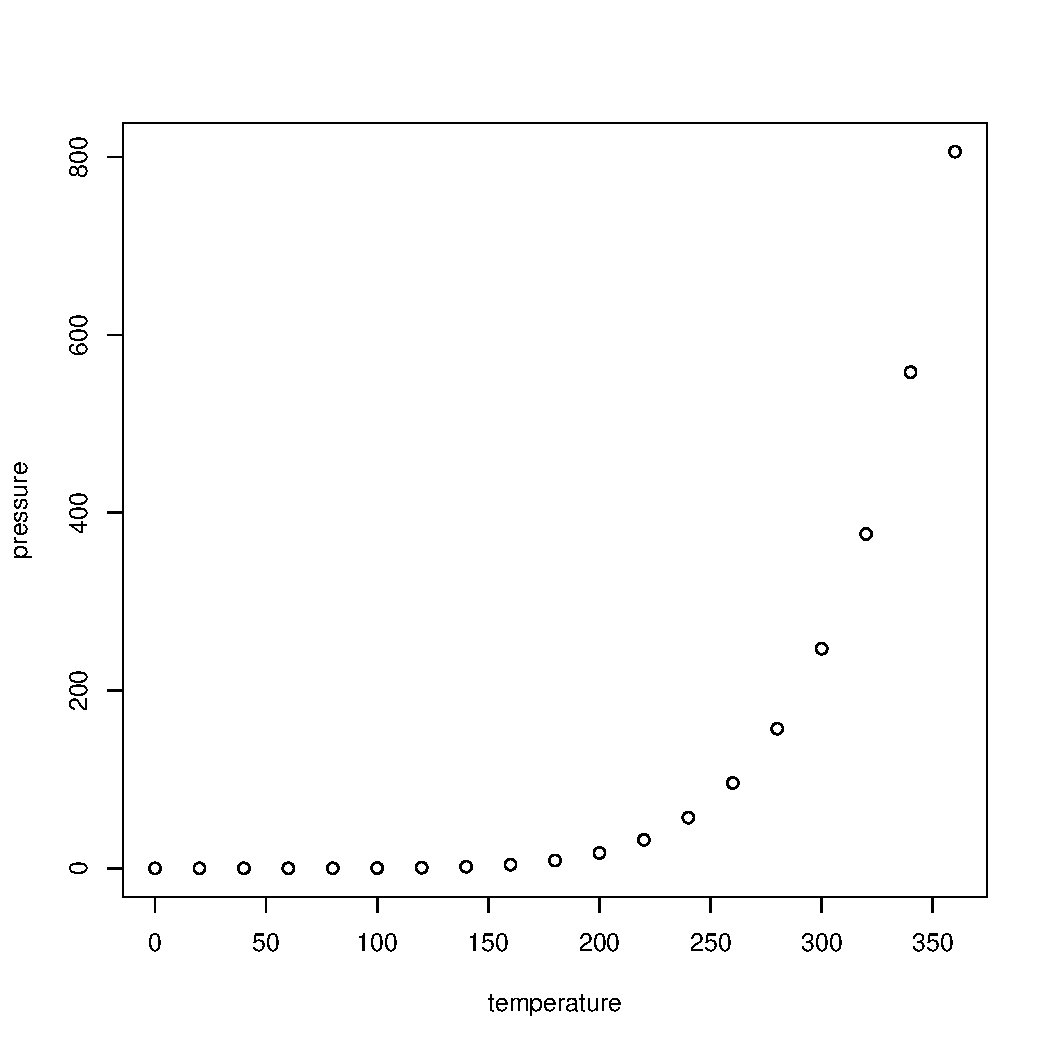
\includegraphics[width=\maxwidth]{figure/fig:pressure-1} 

\end{knitrout}
\caption{Figure Caption...we should turn "echo=False" in the R chunk options, but I left it true for now. (source: ??)} % define the caption, then the label.
\label{fig:pressure}

\end{figure}

\subsection{Floating Figures from External Sources}

All figures and images that are imported should be put into the "images" sudirectory to keep stuff organized. Even better to create a subdirectory with your images, but we can naviagate as we go.

Figure \ref{fig:vadose} is a good example of inserting an image from an external source.

\begin{figure}
\includegraphics[width=\linewidth]{images/Lee-Vadose}
\caption{Vadose zone is neato (Source: \citet{lee2017fifty}).}
\label{fig:vadose}
\end{figure}

In this case, I had to specify the width so it would fit on the page!  See the Rnw file for the code. Notice, I was also abel to ``reference'' the figure in the text.

\section{Adding Citations}

See the Guide, as well, but my video is probably the most helpful.


Generally, there are many environmental trends in Asia \citep{imura2005urban}.

\citet{imura2005urban} describes the how urbanization has affected the hydrology of East Asia. 
 

\chapter{Title...}

\chapterauthor{Nora}

$\rightarrow$

\section{What the Polar Vortex and why do we care?}

\subsection{What Factors Drive Land Use Change?}





\mainmatter


\chapter{The Earth System}\label{earthsystem}

\chapterauthor{Marc Los Huertos}

\section{The Sun's Energy and the Earth's Temperature}

The temperture of the Earth's surface is the result of a balance -- the energy entering the atmosphere and the leaving the atmosphere. Most of this energy is in the form of light or electromagnetic radiation (Figure~\ref{fig:earthbudget}). 

\begin{figure}
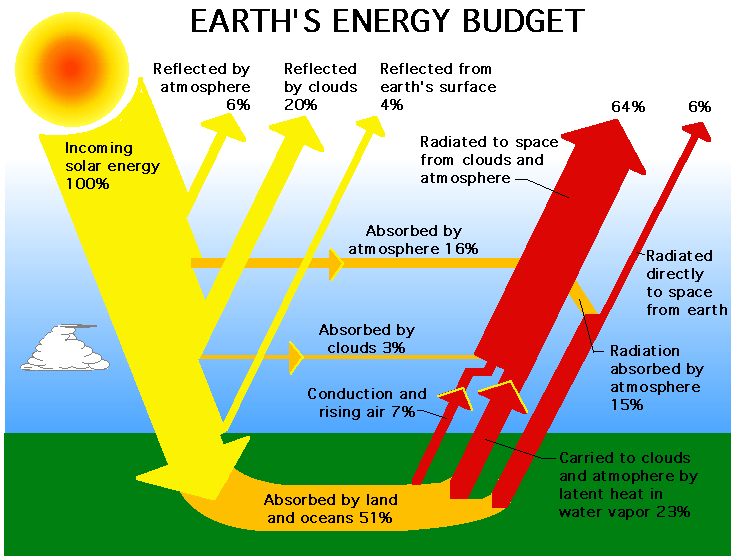
\includegraphics[width=\linewidth]{images/earth-system/earth-rad-budget-nasa-erbe.png}
\caption{caption}
\label{fig:earthbudget}
\end{figure}

Light enters the atmosphere, where some is absorbed and some is reflected. Light interacts in different ways with land, oceans, and vegetation, which is beyond the scope of our project. The ``quality'' of light changes through these processes. 

\subsection{The Spectrum of Light Entering and Exiting the Earth's Surface}

As the sun's electromagnetic radiation interacts with the Earth's Atmosphere, certain wavelengths are absorbed and filtered out (Figure~ \ref{fig:em-entering}).

\begin{figure}
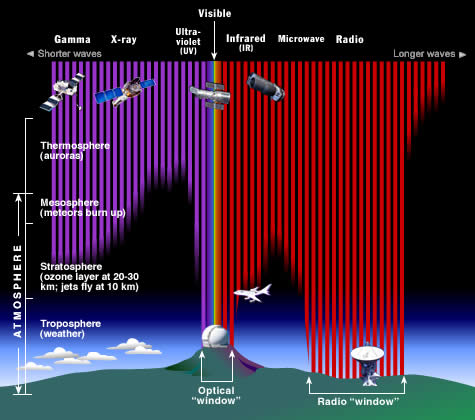
\includegraphics[width=\linewidth]{images/earth-system/em-radiation-atmosph-depth-stsci.jpg}
\caption{Various wavelengths of solar electromagnetic radiation penetrate Earth's atmosphere to various depths. Fortunately for us, all of the high energy X-rays and most UV is filtered out long before it reaches the ground. Much of the infrared radiation is also absorbed by our atmosphere far above our heads. Most radio waves do make it to the ground, along with a narrow `window' of IR, UV, and visible light frequencies. Source: STCI/JHU/NASA.}
\label{fig:em-entering}
\end{figure}

\subsection{The Atmosphere and Greenhouse Effect}



\section{Carbon Biogeochemistry}

\subsection{Long and Short Time Scales}

The carbon cycle processes occur at wide range of temporal scales from hundreds of millions of years to seasons of the year. These have been referred to as long and short carbon cycles. However, for our purposes, I will call them ``geologic carbon'' and ''biosphere carbon'' processes. 

\subsection{Rock Cycle and Geologic Carbon}

The carbon cycle describes changes in the fluxes and reservoirs of carbon in the Earth system. On very long time-scales, millions of years, the primary reservoirs of carbon are the atmosphere, ocean, and rocks (limestone). Carbon moves between these reservoirs through volcanic outgassing, silicate weathering, and limestone sedimentation. The carbon cycle is linked to Earth's energy balance through atmospheric carbon in the form of \carbondioxide, a greenhouse gas.

\subsubsection{Mountains and Erosion}

\ref{fig:carbonpools}

\begin{figure}
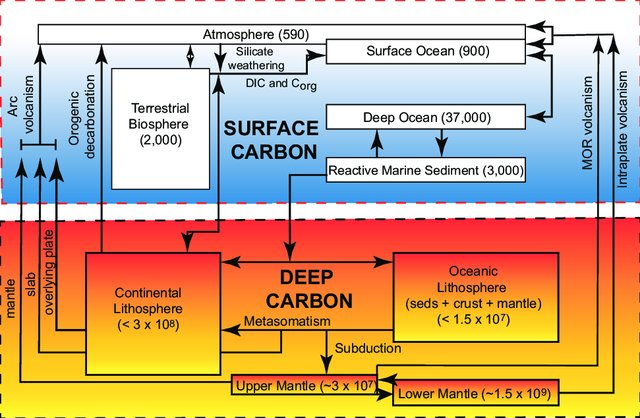
\includegraphics[width=\linewidth]{images/earth-system/Carbon-reservoirs-and-cycles-in-the-Earth.jpg}
\caption{Carbon reservoirs and cycles in the Earth. The figure shows short-and long-term cycles; biosphere and geologic carbon reservoirs and fluxes, and the relative sizes and residence times (y axis) of respective carbon. Numbers in brackets refer to the total mass of carbon in a given reservoir, in Pg C (1Pg C = 10$^{15}$ g carbon). All reservoirs are pre-industrial. Abbreviations: C org = organic carbon; DIC = dissolved inorganic carbon; MOR = mid ocean ridge; seds = sedimentary rocks. Adapted from Lee et al. (2019 And references therein).}
\label{fig:carbonpools}
\end{figure}

\subsubsection{Subduction Burial and Carbon Recycling}

Figure~\ref{fig:longtermcarbon}

\begin{figure}
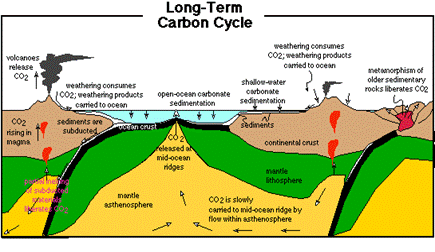
\includegraphics[width=\linewidth]{images/earth-system/long-term-carbon.png}
\caption{Schematic of the long-term carbon cycle (from Bice, 2001)}
\label{longtermcarbon}
\end{figure}

\subsection{Photosynthesis, Respiration, and Biosphere Carbon}

\subsubsection{Soil Respiration and the Soil Profile}

Carbon in soils is respired -- but different pools might have different rates of respiration. Sometimes these pools are distinquished as an active soil organic carbon pool and slow soil organic carbon pool. Although the reference of ``slow'' causes confusion with long-term, geologic carbon, but soil organic carbon remains a component of what we are refering to as biosphere carbon. 

The surface of the soil tends to have more SOC and microbes that can use that carbon for respiration. Lower down in the soil profile, we tend to see lower amounts of SOC and lower microbial biomass (Figure~\ref{fig:soilcarbon}. In addition, soils in the lower part of the profile tend to have more aggregation that protects SOC from microbial attack, thus a key area that soil carbon can seqeustor carbon. 

In addition to these microbial biomass and aggregate patterns, the microbes aree more senstive to temperature changes near the surface as measured by Q10 -- the rate of biochemical processes with a 10 degree C increase in temperature. Thus, soil processes, such as respiration, is likely to increase more near the surface with global warming that the lower part of the soil profile.  

\begin{figure}
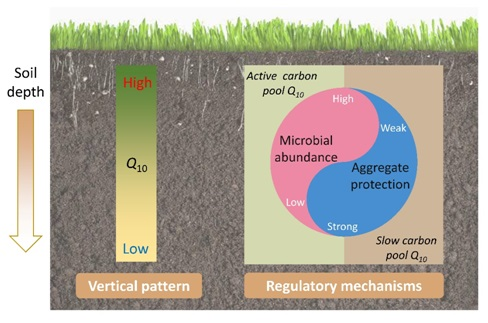
\includegraphics[width=\linewidth]{images/earth-system/Q10-SOC-Regulation.jpg}
\caption{Regulatory Mechanisms of the Temperature Sensitivity of Soil Organic Matter Decomposition in Alpine Grasslands (Source: \citet{Qineaau1218, CAS2021researchers}).}
\label{fig:Q10-SOC}
\end{figure}


\section{Fossil Fuels and Carbon Dioxide Trends}\label{sec:fossilfuels}

As part if the industrial revolution, our energy sources have put more \carbondioxide from the biosphere (soils and forests) and geologic carbon (coal, petroleum). 

\subsection{The Signal of Geologic and Biosphere Carbon in Atmosphere}

The combined contribution from geologic and biosphere carbon in the atmosphere is clearly documented from numerous sources. First, look at data collected at the Mauna Loa where \carbondioxide measurements have been taken continuously since the late 1950s. 

Figure~\ref{fig:maunaloa2}

\begin{figure}
\begin{knitrout}
\definecolor{shadecolor}{rgb}{0.969, 0.969, 0.969}\color{fgcolor}\begin{kframe}


{\ttfamily\noindent\bfseries\color{errorcolor}{\#\# Error in ggplot(train.data, aes(decimal.date, average)): object 'train.data' not found}}\end{kframe}
\end{knitrout}
\caption{Carbon Dioxide Measure on Mauna Loa, HI}
\label{fig:maunaloa2}
\end{figure}






\chapter{Monsoons and East Asia Climates}

\section{Temperature Gradients and Latitude}





\chapter{Critical Zone}\label{ch:critical-zone}

\chapterauthor{Marc Los Huertos}\footnote{The chapter was first drafted by Marc Los Huertos (2021). The author recieved valuable feedback from X, and Y and Z to improve the chapter.}

\section{What is the Critical Zone}

The crticical zone refers the the portion of the Earth's skin where the zone where rock meets life. The Critical Zone supports all terrestrial life.

The critical zone includes the following:

\begin{itemize}
  \item A permeable layer from the tops of the trees to the bottom of the groundwater;
  \item An environment where rock, soil, water, air, and living organisms interact and shape the Earth's surface;
  \item Water and atmospheric gases move through the porous Critical Zone, and living systems thrive in its surface and subsurface environments, shaped over time by biota, geology, and climate.
\end{itemize}

All this activity transforms rock and biomass into the central component of the Critical Zone - soil; it also creates one of the most heterogenous and complex regions on Earth.

Its complex interactions regulate the natural habitat and determine the availability of life-sustaining resources, such as food production and water quality.

These are but two of the many benefits or services provided by the Critical Zone. Such `Critical-Zone Services' expand upon the benefits provided by ecosystems to also include the coupled hydrologic, geochemical, and geomorphic processes that underpin those ecosystems.

\begin{figure}
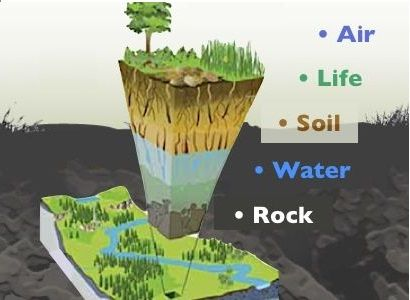
\includegraphics[width=\textwidth]{images/critical-zone/criticalzone.jpg}
\caption{The Critical Zone is an interdisciplinary field of research exploring the interactions among the land surface, vegetation, and water bodies, and extends through the pedosphere, unsaturated vadose zone, and saturated groundwater zone. Critical Zone science is the integration of Earth surface processes (such as landscape evolution, weathering, hydrology, geochemistry, and ecology) at multiple spatial and temporal scales and across anthropogenic gradients. These processes impact mass and energy exchange necessary for biomass productivity, chemical cycling, and water storage.}
\label{fig:criticalzone}
\end{figure}

\subsection{What are the environmental implications of the Critical Zone?}

The critical zone as a concept and as a material space pushes us to think of the porousity of the Earth's surface --- the gas and fluid flows through rocks, soils, and plants. We can begin to appreciate the complexity of the transport and fate of chemical pollutants as they enter the soil and become part of the vadose zone and perhaps the ground water table -- moving with water and diffusing through the water, simultaneously.

\section{Hydrologic Aspects}

\subsection{The Vadose Zone}

Jeji is a volcanic island is located some XX km south of the Korean Penisula. Water runs off the steep slopes quickly and water supplies are limited on the island. To adddress this...\citet{lee2017fifty}.

\begin{figure}
\includegraphics[width=\linewidth]{images/critical-zone/Lee-Vadose.png}
\caption{... (Source: \citep{lee2017fifty}).}
\label{fig:vadose2}
\end{figure}



\chapter{Land Use in East Asia}

chapterauthor{Samantha Beaton}

What is Land Use Change?

What Factors Drive Land Use Change?

How Land Use Change is Measured and Quantified

Integration of sociology

with data science: spatial data compiled from aerial photos, Landsat satellite images, topographic maps, GPS data, etc.

Requires classification and division of land-space types

Ecological Effects of Land Use Change on Soil, Air, and Water

\section{Impacts on Soil}

Deforestation and soil degradation

lack of stability (erosion) and loss of carbon sequestration potential

Forests


coupled with monoculture agriculture

Example Case Study: representative of monoculture agriculture-rice paddies in SE Asia (potentially\ldots)


Impacts on Local Watersheds

hydrology 

infiltration/pollution, groundwater recharge, flow of river basins, runoff

Higher risk of flooding and droughts

\section{Conclusion \& Prospect of Sustainable Urbanization/Land Use Change}


\chapter{Coral Reefs, Ecosystem Services, and Indigenous Peoples}

David Chengwen Gorman

\section{Coral Reef Ecosystem Functioning and Interactions}

\subsection{Coral Reefs: An Introduction}

In November 2018, North Sentinel Island, an island in the Bay of Bengal smaller than 60 square kilometers, drew international attention after its indigenous inhabitants killed an American missionary.  The Sentinelese, one of the last uncontacted people groups in the world, have occupied North Sentinel island for the last 60,000 years. Surrounded by shallow, razor-sharp reefs, the Sentinelese have managed to remain isolated from the rapid development of neighboring Southeast Asian countries and still practice traditional customs and ways of life \citep{Smith}.

This hunter-gatherer tribe is just one of the thousands of Southeast Asian communities that rely on coral reefs for both protection and sustenance. While most do not practice the traditional hunter-gatherer harvesting practices of the Sentinelese, coral reefs remain fundamental to the lives of millions across Southeast Asia. Unfortunately, coral reefs face significant threats and at the current rate of degradation, reef survival is unlikely. The declining health, in terms of biodiversity, biomass, and fitness, of coral reefs impacts not only the overall condition of the global environment, but negatively affects the majority of the Southeast Asian population.

The coral reefs have become vital components of many Southeast Asian, coastal communities and indigenous groups alike. This fragile, colorful marine ecosystem boasts high levels of both biodiversity and biomass, which are vital to both reef survival as well as the millions worldwide dependent on reefs for sustainably and economic prosperity. These life sustaining ecosystems are akin to the rainforests of the sea. There are nearly 100,000 square-kilometers of coral reefs in Southeast Asia supporting 600-800 different coral species. Healthy coral reef ecosystems provide various anthropological benefits, or ecosystem services, to people of all socioeconomic backgrounds. They provide food to over a billion people annually, are a major destination for tourism, and hold great promise for biomedicine. 

As a multi-faceted and dynamic ecosystem, the reefs are constantly changing. They face countless threats and stressors, including the effects of climate change, pollution, and overfishing; the reefs are struggling. General reef health serves as an indicator for both global and marine ecosystem health, and unfortunately, the easily observed reef degradation is representative of many other ecosystems worldwide \citep{RAR}.

This chapter describes coral reef ecosystems and current environmental and anthropocentric threats to coral reefs in Southeast Asia.  Because of reefs high value to Earth and indigenous groups, conservation is essential; reef restoration efforts will also be highlighted. The following sections will detail the dynamics, threats, and benefits of the Southeastern Asian coral reefs, while focusing on indigenous interactions and their reef reliance.

\subsection{Coral Functioning}

Coral polyps are tiny animals that work together by the thousands to build reef ecosystems. Each coral polyp uses calcium and carbonate ions that have been dissociated in the surrounding water to create calcium-carbonate (limestone) skeletons. During the day, these vulnerable, nocturnal creatures protect themselves by hiding in their limestone skeletons. At night, they extend their many tentacles to feed, using specialized cells called nematocysts to stun their prey before consumption. Coral polyps are part of the family Anthozoa, which includes sea anemones as well, explaining their similarities. Most species of coral are extremely slow growing, and the majority grow by less than an inch every year \citep{coralreefalliance_2021}.

The majority of corals, and the ones more important for the reef ecosystem, are classified as hard corals. These corals are reef-building corals, or hermatypes. They create the calcium carbonate skeletons which support the coral reef ecosystem. The shape of these skeletons, while heavily influenced by genetic composition, is also largely dependent on the surrounding environmental conditions to which the coral is subject. In rougher water with stronger waves breaking over the reefs, hard corals tend to create a more robust, stable shape, like a mound or coral flat. In contrast, corals in more sheltered, calmer waters can create complex shapes with intricate branching patterns \citep{coralreefalliance_2021}.  

The body of each coral is actually clear; the intricate colors come from single-celled dinoflagellates, or plant cells living inside the corals. This grouping of small, photosynthetic algae living in symbiosis with the coral polyps are generally referred to by their colloquial, zooxanthellae. \citep{noaa}. These algae grow inside the coral and photosynthesize, providing the necessary nutrients and oxygen the coral needs to grow and survive. The coral protects the zooxanthellae with its calcium-carbonate skeleton, and via respiration, provides the carbon-dioxide needed for photosynthesis. This symbiotic relationship between coral and algae is delicately balanced, and small disruptions can have catastrophic effects not only for the organisms involved, but also for the entire ecosystem as a whole. \citep{https://doi.org/10.1002/fee.2088}  

Corals are incredibly slow growing, as they require a delicate balance of nutrients and environmental conditions. Most species only grow between 0.2-1 inch per year. Coral reproduction processes vary by species. Some coral species are hermaphrodites, able to produce both eggs and sperm at the same time. Others are gonochoric and can only produce one of the two gametes. Coral larvae can be formed either inside the polyp body or outside the polyp body, such as during mass gamete ejection events. Coral larvae are released into the water, where they are free swimmers. They first swim to the surface, and then fall back to the seafloor where they must attach to a hard surface, like a rock or preexisting coral skeleton. Once attached, the corals begin dividing and making genetic copies of themselves. They then can begin secreting the calcium carbonate skeleton, which in turn attracts zooxanthellae, and the symbiotic relationship begins \citep{coralreefalliance_2021}.

For the duration of this chapter, the term ``coral'' will be used to describe the network of polyps which comprise the visual structures of the reefs. 

\subsection{Reef Organisms and Trophic Interactions}

The species the reef ecosystem largely depends on, or its keystone species, are the coral polyps. They provide the entire structure and habitat from many reef-dwelling creatures with their calcium carbonate skeletons. The coral polyps themselves constitute a small percentage of the total biomass of the ecosystem, as the average coral polyp is only around 1.5 cm large, yet their impact is vital to the ecosystem's survival. Many species depend on these coral skeletons for either protection or as hunting grounds. Fish, invertebrate, and other organisms aggregate around these underwater structures, accounting for the ecosystem’s dense biodiversity and high overall biomass. Some argue that the Parrotfish is another, secondary keystone species. This herbivorous fish eats algae latched onto the coral skeletons, which blocks sunlight and limits the photosynthetic abilities of the zooxanthellae. In a sense, its niche is to ``clean the coral,'' allowing normal function to continue. The Parrotfish is a highly targeted, overfished species, and because it fulfils an important niche, its removal negatively effects the entire reef ecosystem. This specific niche is just one of many, all which illustrate the complex relationships involved in the coral reef ecosystem and the importance of each species to the ecosystem \citep{https://doi.org/10.1890/15-1492.1}. 

These relationships can be further illustrated by an examination of the indirect actions which affect entire ecosystems and stem from trophic-level suppression, known as trophic cascades. For Southeast Asian reefs, the most prolific trophic cascade exists between urchins and the orange-lined triggerfish. The triggerfish is a keystone predator and limits uncontrolled urchin expansion. Without these predators, urchin populations would explode and consume everything on the seafloor, creating urchin barrens incapable of supporting life. These predator-prey interactions are disrupted by anthropocentric activities, mainly overfishing. As the fish are removed from the ecosystem at an unsustainable rate, the detrimental grazer effects of the urchins are exacerbated. While negative human influences will be discussed in future sections, this illustrates how interconnected reef species are the delicate equilibrium between them \citep{https://doi.org/10.1890/15-1492.1}.

\subsection{Necessary Climate and Nutrients}

Coral reefs require a delicate balance of nutrients and external conditions, which is easily upset, making them especially vulnerable. As for physical needs, sunlight is a crucial limiting factor of the ecosystem. The zooxanthellae require shallow waters with low turbidity, or high clarity. This means they generally can only survive in waters under 50 meters, mostly free of sediment and debris. The water also cannot have too many nutrients, as explosive algae growth can cloud waters and block the necessary sunlight needed for photosynthesis. Corals reefs exist in tropical climates usually, as they also need warmer waters of around 20-32 degrees C (68-90 degrees F). This explains the abundance of coral reefs in the tropical, warm climate of Southeast Asia. Finally, corals need water with a high salinity, or saltwater concentration. They cannot survive in brackish water or estuaries, or anywhere where freshwater sources like rivers drain into the ocean \citep{https://doi.org/10.1002/fee.2088}.

FIGURE

\subsection{Southeast Asian Reefs by Country}

MAP
TABLE

\section{Climate Change and Its Effects on Coral Reefs}

\subsection{The Indigenous Paradox}

Climate change and global warming are undoubtedly one of the biggest contributors to the loss of biodiversity and overall destruction of coral reefs. The IUCN Red List Index (RLI), a comprehensive list tracking biodiversity loss and extinction risk, identifies corals as one of the fastest declining species (in terms of diversity and richness) in response to climate change \citep{wwfindex}. Even all localized reef threats and pollutants were eliminated, the overarching threats of ocean acidification and rising temperatures hold the ability to eradicate reefs entirely \citep{Keller2009ClimateCC}.

In addition to reef eradication, climate change disproportionately effects lower socioeconomic classes, specifically, indigenous people groups. Many Southeast Asian indigenous coastal peoples are reliant on reefs not only for food and sustenance, but they also have strong cultural ties to the reefs and surrounding waters. Climate change threatens these indigenous people-reef ecosystem interactions, and these threats compound other climate change-associated dangers affecting indigenous groups. As many indigenous groups inhabit harsh and isolated environments, they are highly vulnerable to the rising sea levels and increased storm severity resulting from climate change. They are also often excluded from policy discussions and legislative responses to climate change, further increasing their susceptibility to climate change disturbances \citep{13772149520190801}.

	Oddly, indigenous groups are some of the most well-adapted and resilient groups in response to climate change as well. Knowledge of specific environments and ecosystems is passed down generationally, creating a plethora of knowledge concerning responses to environmental issues, all which can be used to combat the effects of climate change. This ecosystem expertise and resilience, coupled with their high vulnerability to climate change, creates what some call ``The Indigenous Paradox.'' Indigenous groups all throughout Southeast Asia are continually ransacked by reef degradation in response to climate change, yet their complex, generational knowledge is vital in combatting climate change and reversing its current narrative. Indigenous peoples offer highly valuable resources concerning reef restoration, which will be discussed further in Section \ref{sub:ie} \citep{13772149520190801}.

\subsection{Rising Sea Level}

A primary issue when discussing climate change and the ocean is rising sea levels. This is due to both melting polar ice caps and thermal expansion of water molecules caused by the rapid increase in temperature, or thermal heat, in recent years. Sea levels are projected to continue to rise 0.5-1.5 meters by 2100, undoubtedly impacting both submerged ecosystems and coastlines worldwide. \citep{coralreefalliance_2021}.

Brian Keller, regional Science Coordinator of NOAA's Office National Marine Sanctuaries, and his colleagues conducted a study concerning sea level rise and its effect on corals on the Sanya Bay of the South China Sea, where they discovered a potentially unforeseen positive development: the sea level rise promoted coral growth. The previously degraded reef was able to recolonize via asexual fragmentation in response to the 16.2 ± 0.6 cm rise over the previous 30 years. Of the corals the study surveyed, 86\% were under 30 years old, suggesting that the rise in sea level promoted their growth. Theoretically, this makes sense. Sea level rise increases the vertical space a coral can grow in, or the accommodation space. As the coral gets closer to the surface, growth is inhibited by temperature, exposure, and sediment, but by increasing the overall depth, growth can occur in a greater area of water. At first glance, this promising result suggests that climate change actually may benefit coral reefs in some way, but that is unfortunately not the case. Only specific coral species are suited for a rapid rise in accommodation space, which may select out other species. This leads to an increase in total growth but a decrease in biodiversity, and with organisms as vulnerable as coral, biodiversity is crucial \citep{https://doi.org/10.1029/2018JC014534}. Retrospective studies have also found that coral growth rates increased with sea level rise over 16,000 years ago, and then faltered as the sea level became stabilized during the Holocene (current time period, which began 11,700 years ago), but these results cannot be taken as indications of future outcomes. Coral growth capacity is likely to be inhibited by other factors, both regional and global, so an increase in accommodation space may have negligible overall impact \citep{Keller2009ClimateCC}.

The negative effects of sea level rise on the coral reef ecosystem are relatively unquantified, yet practically accepted as true based on past events and prospective insight. Rising sea levels pose risks to coastal regions, with the threat of washing entire communities into the ocean.  Such catastrophic events would undoubtedly add sediment and pollutants to the water while also physically damaging corals and other organisms with the marine debris. Community submergence would also displace people groups, causing them to either move inland or to other coastal areas. Many would likely move to other coastal areas to practice similar lifestyles, which would in turn concentrate pressure on reefs not yet affected by coastline degradation. Indigenous groups and other coastal communities are disproportionately threatened by sea level rise, as the already underrepresented groups will be forced off their land now not only by oppressive governments and corporations, but also by nature itself. These threats to coral reefs may seem distant, but they are quickly approaching realities imposed by climate change \citep{Keller2009ClimateCC}.

\subsection{Ocean Warming and Acidification}

Climate change has already begun to negatively impact reefs in quantifiable ways that can be observed at the molecular level. Fossil fuel emissions release carbon dioxide into the atmosphere, and a third of that gas is absorbed by the ocean\citep{Keller2009ClimateCC}. As carbon dioxide dissociates, it releases protons, which when added to the water, lowers the pH, making it more acidic. Since the Industrial Revolution, a 0.1 pH drop has been observed on the ocean surface, and this drop is expected to increase as global emissions continue and CO$_2$ concentrations rise. In more acidic conditions, corals struggle to efficiently create their hard skeletons \citep{Keller2009ClimateCC}. The carbonate ion saturation, or aragonite saturation, is crucial for skeletal growth, as the carbonate ion is one of the two necessary ingredients needed for limestone formation. The bicarbonate ion formed by the carbonic acid-carbonate interactions is unusable to corals, thus slowing skeletal growth (see figure for complete chemical process). It is estimated that up to 60\% of reefs today persist in waters with inadequate aragonite saturations \citep{Ayala_2009}.

The skeletons built by corals in waters lacking proper carbonate ion concentrations not only form slower but are also weaker and less robust.  As a result, corals have fewer defenses to fight pressures and, combined with the slowed growth rates, may not be able to overcome the pre-existing stressors they face. Increasing acidification will likely cause coral production rates to fall below destruction rates, decreasing reef size and affecting the ecosystem as a whole. Additional stress from acidification and climate change only adds more threats to coral, creating a detrimental positive feedback loop for the already struggling polyps \citep{Ayala_2009}.

On top of ocean acidification, as greenhouse gas emissions continue to cause earth’s surface to warm, the ocean warms with it. This rise in temperature is the main cause of sea level rise, due to both glacial melt and the molecular expansion of water molecules in response to heat. Ocean warming and its effects on coral reefs is still a topic requiring more research, but its effects have already begun to be observed \citep{wwfindex}.

Coral disease transmission is exacerbated by higher temperatures, which will be explored further in Section \ref{sub:cd}. Unusually high-water temperatures are the main cause of coral bleaching, and as ocean temperatures continue to rise, mass bleaching events are expected to increase in both frequency and severity\citep{Keller2009ClimateCC}. It is generally agreed that ocean warming will have disastrous future effects on coral reefs.  In 2018, Intergovernmental Panel for Climate Change, or IPCC, reported that a mere two-degree Celsius rise in temperature will completely eradicate the coral reefs, with an estimated loss of around 99\% of reefs worldwide \citep{wwfindex}. 

\subsection{Coral Bleaching}

Coral polyps react to warming water temperatures and other environmental stressors by expelling their algae. If the waters do not cool or the stressor continues to persist, the algae will not come back, and the coral will starve without them. The starved corals crumble into empty, white, lifeless skeletons. This is known as coral bleaching, and it has the potential to destroy entire reef ecosystems in an alarmingly short period of time \citep{https://doi.org/10.1111/gcb.14871}. 

Most bleaching and mass coral mortality events are driven by heat waves, which have increased with climate change and global warming. The disruption of the coral-algae symbiosis caused by the loss of algal endosymbionts is what causes the corals to pale, as the algae are responsible for coral coloring. Without their symbiotes, the corals lose the ability to feed and rapidly starve and die off. Not only does this halt further reef growth, but it also sends negative ecological cascades throughout the ecosystem. Many organisms' habitats are destroyed as the coral, the keystone species and ecosystem engineers, are removed \citep{https://doi.org/10.1111/gcb.14871}.

Coral bleaching is the net outcome of complex, multifactorial stressors working at both the cellular and ecosystem levels. At the cellular level, the accumulation of reactive oxygen species, or ROS, triggers signaling cascades prompting corals to expel their zooxanthellae. These ROS are both produced and accumulated in response to environmental changes and stressors. At the ecosystem and environmental level, the most common stressor is heat waves. The first-ever observed mass coral bleaching event in 1998 was driven by El Niño, and rising temperatures have been accredited with the increasing frequency of bleaching events. The two recent back-to-back bleaching events in both 2016 and 2017 show not only the vulnerability of the coral ecosystem to change, but also how climate change will only make coral bleaching more frequent and of greater severity. Other environmental exacerbators include, but are not limited to, light availability, salinity, oxygen demand, organic nutrient availability, and inorganic nutrient availability. While one of these single factors may not cause a mass bleaching event, they are interconnected and have cumulative effects on the fragile, not-easily-adaptable coral polyps. Each factor also can change how well coral adapts to rapid heat change. Coral bleaching is the result of a complex, dynamic system that global warming negatively affects in multiple ways \citep{https://doi.org/10.1111/gcb.14871}.

\section{Unsustainable Fishing Practices}

\subsection{The Live Reef Fish Trade}

Unsustainable fishing practices are arguably the most detrimental local practice to Southeast Asian reefs. Over 55\% of reefs worldwide are affected by overfishing and unsustainable fishing techniques, and this number is higher in Southeast Asian reefs. Overfishing disrupts food web balance, since macroalgae, without as many fish as predators, grow disproportionality and smother corals. Overfishing has made fish harder to catch, leading to a shift away from sustainable fishing practices. Unsustainable fishing threatens not only fish stocks and ecosystems, but also local economies and the people that rely on fish for food. The methods currently used to catch live fish, like cyanide fishing or blast fishing, have been incredibly destructive to the coral reefs of Southeastern Asia. Both Indonesia and the Philippines offer textbook examples of unsustainable practices which still persist today, despite efforts to regulate and ban them \citep{coralreefalliance_2021}.

A major driver of unsustainable fishing practices is the Live Reef Fish Trade, or LRFT, which is precisely as it sounds: selective fish are caught alive and sold as high-priced delicacies. Certain high-commodity fish, like leopard coral reef fish, are targeted and fished for disproportionately, selectively pressuring reef ecosystems and disrupting trophic interactions. These fish can sell for as much as \$60 USD per kg instead of the average \$2 USD per kg for most fish. In locales such as Palawan, Philippines, where the average monthly income is under \$100 USD, it is no surprise the LRFT would flourish. Fishermen explain,``It's like hitting the jackpot every time'' \citep{10.2307/40603032}. 

Many of the practices for catching live fish are inherently destructive. Fish are often caught young and then grown to an edible size. This excessive juvenile capture removes fish before they can reproduce and contribute back to the ecosystem, further reducing the fish stocks of the selected species. Other more violent methods, like cyanide and blast fishing, have horrid effects on reefs, and these will be discussed in the following sections \citep{10.2307/40603032}.  

The LRFT has continued to grow in both the Philippines and Indonesia despite both decreasing profitability and fish stocks. This dangerous combination has led to high levels of overfishing that further destroyed coral reefs. Fishermen are catching less fish and must travel farther distances to find them, causing large scale economic losses in both coastal communities and the individuals residing in them. Because the LRFT is poorly regulated and any existing regulations are often not enforced or disregarded, the harmful impact of the LRFT is likely to continue \citep{10.2307/40603032}.

\subsection{Cyanide and Blast Fishing}

The selective catching of live fish is easily accomplished through the use of sodium cyanide, which stuns larger fish to be later revived. While it may sound complex, cyanide fishing is as simple as diving with a spray bottle containing crushed sodium cyanide tablets which can be injected into reef crevices or squirted directly into the faces of desired fish. While larger animals may only be stunned and can later revive, smaller organisms are severely poisoned by the cyanide, as it represents a much larger proportion of their body weight and size. These animals inevitably die, disrupting ecosystem functioning on multiple levels. Cyanide is most often fatal to small fish, invertebrates, corals, and their symbiotic algae \citep{wwfcyanide}.

	After just 30 seconds of cyanide exposure, coral becomes stressed and begins to lose its ability to function normally. It is estimated that for every live fish caught with cyanide, a square meter of reef is destroyed. Cyanide fishing is not only used for the LRFT, but also for aquarium trade as well. At the turn of the century, 75\% of all aquarium fish coming from Southeast Asia were estimated to be cyanide-caught. It is estimated that around two-thirds of all Filipino reefs are affected in some way by cyanide poisoning \citep{970313024119970301}.

Despite being banned in both Indonesia and the Philippines, cyanide fishing still persists today. Asia’s growing affinity for live fish, with neighboring countries like China and Hong Kong making up the majority of the market, fuels the continued use of cyanide fishing. The Padilla region in the Philippines is responsible for around two-thirds of all live fish exports, exporting up to a ton of fish per day. Many of these live fish are caught via cyanide fishing. The minimal regulations and negligible punishments for cyanide fishing enable this destructive practice to continue. There have been almost no convictions or case files against cyanide fishing—only six total have occurred in six years \citep{wwfcyanide}.

FIGURE

Blast fishing is another way to stun fish for the live trade harvest. Explosives are detonated in reefs to stun fish, which are then selectively chosen for live trade. Like cyanide fishing, smaller organisms are often immediately killed by these blasts, and the coral is as well. Because blasts also break the preexisting coral skeletons, both the habitat and entire ecosystem are destroyed.  Over half of all Southeastern reefs are threatened by blast fishing practices \citep{https://doi.org/10.1890/1051-0761(2006)016[1631:RFBFOC]2.0.CO;2}. 
  
The explosives used are almost always homemade and can be as simple as a kerosene-fertilizer mixture inside a glass soda bottle. Just one 300mL bottle can create an explosion which leaves behind a crater with a 1-meter radius capable of lasting multiple years. Besides the general fatalities from the blasts, one of the biggest issues associated with blast fishing is the leftover coral skeleton debris. An examination of craters left behind by blast fishing concluded that even after five years, the rubble and debris left inside the crater was between 5-10 cm deep. This additional sediment can smother both coral and algae, either blocking light and hindering photosynthesis or burning still-intact corals alive. Larger debris and skeletal pieces can also abrase growing corals, scraping off growing colonies or hindering recruitment by blocking secure surfaces for attachment \citep{https://doi.org/10.1890/1051-0761(2006)016[1631:RFBFOC]2.0.CO;2}. 

Over half of all Southeast Asian reefs are currently threatened by blast fishing practices. Again, like cyanide fishing, blast fishing is legislatively banned, but this ban is not adequately enforced. Blast fishing was banned in Indonesia in 1985, yet it still continues today, not only in Indonesia, but also in most other reef-bearing Southeastern countries \citep{https://doi.org/10.1890/1051-0761(2006)016[1631:RFBFOC]2.0.CO;2}. 


\subsection{Economic Drivers and Indigenous Contributions}

A group of indigenous peoples deeply impacted but also highly connected to unsustainable reef fishing is the semi-nomadic, boat dwelling communities of Southeast Asia. These maritime communities are reliant on the sea for subsistence, often inhabiting areas of high biomass and biodiversity, as resources are often concentrated there. As a result, many of these communities are situated near coral reefs and rely on them; to them, reef survival means human survival \citep{boatpeople}. 

One of these groups, the Sama-Bajau, reside mainly in the Philippines and eastern Indonesia. Foods derived from reefs provide a majority of their protein intake, and fishing is a dominant economic sector among the group. Most other economic activities among the Sama-Bajau relate to reefs, as reef reliance supports a wide range of activities, from boat building, to guiding tours, to sea trading. Many groups like the Sama-Bajau have modernized to incorporate stilt houses, giving them more of a sense of community and stability. Unfortunately, many other groups lack government representation, and in turn cannot officially own land areas for settlement. The resulting highly mobile lifestyle deprives these groups of not just landownership, but also healthcare, education, and traditional economic prosperity \citep{boatpeople}.

Because of the many factors contributing to indigenous suppression and poor socioeconomic conditions, the vast majority of the reef fishermen are poor and struggle to sustain themselves and their families through traditional fishing practices. One factor of interest is the drop-out rates among children in these indigenous groups. The reef-reliant, seafaring lifestyle is commonly not respected among upper socioeconomic classes, for these indigenous groups are viewed as primitive and uncivilized. As a result, indigenous children face widespread racial and cultural discrimination, leading them to drop out of school and pursue a less economically prosperous career, like fishing. As reefs are continually degraded by overarching issues, such as climate change and local issues (e.g., corporate overfishing and pollution), sustainable fishing practices become less viable. Many Sama-Bajau fishermen, like other indigenous fishermen, have turned to the more lucrative unsustainable fishing practices like blast fishing and cyanide fishing. Driven by the high demand of the LRFT and aquarium trade as well, these destructive fishing practices promise steady, higher payouts than traditional fishing methods. Indigenous participation in these activities is not driven by economic greed, but purely because they lack other alternatives to feed their families. These fishing practices further degrade reefs, putting indigenous groups in a viscous cycle of reef degradation and economic activity loss. The drivers of many of the previously mentioned unsustainable fishing practices result from a complex system of oppression, especially among indigenous groups of Southeast Asia \citep{boatpeople}.

\section{Reefs Pollutants}

\subsection{Marine Debris and Ocean Contaminants} \label{sub:mdoc}

A significant number of anthropocentric activities contribute to reef pollution. Pollutants can be classified generally in three categories: toxins, sediments, and nutrients. Toxins cause physical harm to corals and other organisms at the cellular level. They can be organic or inorganic and are often found in chemical runoff. Sediments block sunlight and prevent photosynthesis and limit primary production. They also reduce the number of viable locations for coral larvae to attach to, as the loose sediment settles on the previously secure spots on the coral skeleton. Sediment also increases the turbidity of the water, blocking visibility. This can contribute to biodiversity loss, selecting for certain animals which do not primarily rely on eyesight. Finally, nutrients can promote algal blooms which smother corals, or they can disturb organismal balances within the ecosystem, disrupting critical interactions among populations. Nutrient increase, or eutrophication, can also promote pathogenic growth among corals and lead to coral epidemics. A wide range of human activities contribute to reef pollution, with globalization, population expansion, and development as main exacerbators \citep{4884777420100401}.

Marine debris is essentially human trash, which enters the water via boats or from land. Floating trash can bear resemblance to jellyfish and is often consumed by animals, obstructing their gastrointestinal intestinal tract \citep{coralreefalliance_2021}. If not eaten, it also may snag corals and shade them, so that the zooxanthellae cannot adequately perform photosynthesis, and thus starving the corals. This trash entanglement also may break off chunks of coral, killing entire colonies \citep{USEPA_2017}. Lost nets, lines, and other ghost fishing gear also often entangle corals and other reef organisms, severely hindering their mobility and often killing them. The levels of marine litter in Southeast Asia generally exceed the global average, with new coastal development, ineffective regulatory methods, and heavy shipping traffic throughout the region being main contributors \citep{4884777420100401}.

The majority of marine trash is plastics, which account for 60-80\% of all marine litter. Plastics take multiple generations to degrade and can act as a skin for chemical pollutants, carrying chemicals and toxins into the water from the land or anything else they were in contact with. At each successive trophic level, plastic can be ingested, as there is significant variation among the size of plastic particles. Plastics travel up the entire food chain, decreasing both energy reserves and feeding capacity. Plastic ingestion also decreases the ability to produce offspring, or fecundity. Oceanic plastic pollution is so high that it is estimated there is not a single ocean organism that is completely unaffected by plastic ingestion, either directly or indirectly \citep{12907334620180601}.

The traditional ``plastic pollutant'' is a macroplastic, that is, visible to the naked eye. In actuality, microplastics, or plastic particles under 5mm, comprise the majority of plastic pollution and are increasing in concentration at alarming rates. These microplastics can enter the surrounding reef waters as fragments from larger plastic debris or in terrestrial runoffs and waste dumps. They affect different species of coral differently, but each varying effect is almost always negative. They may attach to corals and disrupt cellular functioning, or they can cause excessive mucus production and overgrowth. Microplastics are small enough for corals to ingest, and the corals retain the plastic fragments for extended periods of time. Microplastic exposure may trigger signaling cascades related to cleaning and digestive responses among different coral species. In a microplastic-coral interaction study, five out of the six coral species examined displayed serious negative health effects when exposed to microplastics. In areas with higher concentrations of microplastics, bleaching and tissue necrosis was widely observed. Microplastic exposure is continually increasing, and poses a serious threat to reefs, corals, and reef organisms alike \citep{12907334620180601}.

Both sewage and wastewater discharge contribute a significant amount of toxins and contaminants to reef water. Chemicals, toxins, bacteria, and pathogens can enter reef ecosystems from cesspools, septic tanks, landfills, sewage treatment plants, and more. These chemicals have obvious negative effects on coral reefs, as many of them can either kill or infect corals and reef inhabitants \citep{coralreefalliance_2021}. In Southeast Asia, over 80\% of sewage deposited in the ocean is left untreated, inevitably depositing high levels of toxins and chemicals into the waters \citep{4884777420100401}. One of the most prevalent chemicals affecting coral reefs, however, comes not from industrial waste and sewage, but from tourists and everyday people. Oxybenzone is a common component of sunscreen, which enters the water whenever people wearing sunscreen do. Along with other harmful chemicals in sunscreen, oxybenzone damages coral DNA and also accumulates in tissues, either causing death and deformities among adolescent coral colonies or inducing bleaching \citep{USEPA_2017}.

Another major source of reef contamination is crude oil, which blocks sunlight, smothering and starving reefs. Oil enters the ocean not only though spills, but also via operational discharge. This oil itself contains toxic components. One of these substance groups, polycyclic aromatic hydrocarbons (PAH), bind to coral DNA and proteins, and in turn disrupt necessary cellular functions \citep{4884777420100401}. While the oils themselves are harmful, the dispersants used to clean up spills are actually more damaging to coral polyps. Surfactants and other solvents are often used for their ability to dissolve and break apart large floating sheets of oil into smaller droplets. These dispersants are toxic to coral larvae and can kill large sections of young coral fairly quickly. They also prevent the fertilization of mature eggs and hinder coral maturation, or metamorphosis. Oil contamination and surfactant poisoning are increasing in Southeastern coral reefs, as development has continued to increase in Southeast Asian coastal regions \citep{2615280620070801}.

\subsection{Development, Industrialization, and the Agta}

Many coastal regions in Southeast Asia have seen rapid development in the past couple of decades. This development in itself has negative effects on reefs, as piers and other structures are often built on top of already struggling reefs, negating any chance of regeneration. Resources like sand and limestone are also sometimes extracted from reefs in a process called coral mining; large coral pieces and other reef materials are used as road fills, bricks, or cement components \citep{coralreefalliance_2021}. Much of this coastal development also releases high concentrations of sediment into the water, increasing turbidity and primary production within the reef. Coral reefs are continually polluted by the dredging, dumping, and shipping all associated with development as well. While development is typically a positive economic indicator, it often carries disastrous environmental side effects, as evidenced by the relationship between development and the coral reefs \citep{USEPA_2017}.

Road construction in particular generates many negative consequences for reef growth and survival. Not only does road construction release high levels of toxins into surrounding waters, but it also adds a great deal of sediment as well. Roads, as well as other impervious structures, do not allow liquids to seep into the soil. Instead, they flow across road surfaces and downward, generally towards sources of water. Even after construction is complete, runoff from coastal roads continue to contribute substantial amounts of toxins and sediment to the reefs. This is especially problematic during storms and in areas of high precipitation, as heavy rains pick up toxins and sediments from the ground and flow via roads directly into the ocean. Both Indonesia and the Philippines host monsoon climates, and because this stormwater cannot be filtered by the soil, it carries all of its pollutants into the reefs. Notable toxic substances reaching waters in greater quantities include metals like lead or mercury or organic chemicals like polychlorobiphenyls (PCBs). This particular carcinogenic dioxin not only takes a long period of time to break down, but also affects the growth rates, feeding patterns, defensive responses, and reproductive processes of all coral species. As road, industry, and urban development persist, the runoff will continue to carry chemicals, toxins, sediment, nutrients, and pathogens into surrounding reef water \citep{USEPA_2017}.

In addition to reef degradation, development and industrialization has often displaced indigenous groups. Development indirectly undermines indigenous groups by harming reefs, but also directly hurts them via displacement and relocation. One of these groups, the Agta people of Northeastern Luzon in the Philippines, perfectly exemplify this scenario. Over the past decades, infrastructural development has displaced many of the Agta, forcing them to live as landless peasants on the outskirts of other towns and villages. Much of the Agta lifestyle consists of spearfishing the shallow reefs of their native waters, and as they are pushed further inland, they cannot continue their traditional practices. Instead, they must adopt different livelihoods, and turn away from their ancestral reef reliance, breaking the longstanding cultural ties and connections to the water \citep{RePEc:gam:jsusta:v:12:y:2020:i:19:p:7983-:d:420111}.

\subsection{Deforestation and Agriculture}

As the Agta are continually forced inland, they must find new economic activities to sustain themselves. The most commonly chosen new livelihood is small-scale, swidden agricultural cultivation. Slash-and-burn technique is used to clear areas for farming, contributing to both deforestation and agricultural issues in the near-coastal forests. Both are contributors of reef pollutants, further harming the already struggling reef ecosystems and the other indigenous coastal groups who still rely upon them \citep{RePEc:gam:jsusta:v:12:y:2020:i:19:p:7983-:d:420111}.

Deforestation adds high levels of sediment into the surrounding waters, smothering coral. Corals and their endosymbionts in sediment-filled water cannot carry out nightly respiration or daily photosynthesis in an efficient manner. In Indonesia, palm oil plantation growth is a major contributor to deforestation, while in the Philippines, the expansion of logging and agriculture industries is the main cause. In both countries, corruption, poor regulation, and economic greed have exacerbated this issue. One specific tree of interest is the mangrove, which is particularly important to reef protection. Many reef fish raise their young in the protected labyrinth of the mangrove forest, and without it, many offspring become easy prey. In addition to the traditional consequences of deforestation, mangrove destruction also means nursery loss. Mangrove forests also act as filtration systems for sediment, and without them acting as a barrier, more sediment from runoff and other human activities reaches reefs. Three quarters of the mangroves in the Philippines have already been lost, and as agriculture continues to expand, this number is likely to rise \citep{coralreefalliance_2021}.

	Agricultural runoff also adds sediment to reef water, but more importantly, agricultural runoff adds excess nitrogen, phosphorus, and other nutrients. Generally, having more nutrients is beneficial, but the reef ecosystem is adapted to survive only at specific, lower-nutrient levels. Nutrient excess selects for other organisms like seagrass, however, which boom in population and outcompete corals for their required nutrients. This eutrophication stems mainly from runoff and discharge containing manure, fertilizers, aquaculture byproducts, and pesticides. Manure and other fertilizers cause phytoplankton booms which not only block sunlight but can also create toxins that are dispersed throughout the ecosystem. These massive algae blooms also require tremendous oxygenic support, causing hypoxic conditions in the water surrounding them. The already struggling organisms often succumb to hypoxia and die off in mass quantities. When pesticides reach the waters, they generally disrupt the symbiotic coral-algae relationship. Herbicides in particular are very dangerous, as they kill the algae and induce bleaching. Finally, when corals are exposed to too many nutrients, bacteria and other pathogenic growth are promoted. Diseases and coral contamination quickly follow \citep{4884777420100401}.

\subsection{Coral Diseases}\label{sub:cd}

Corals are highly susceptible to diseases. They lack virtually any dispersal barriers and spread rapidly due to how close in proximity coral colonies are to each other. Viruses, bacteria, and fungi can cause diseases among coral species, which all proliferate with temperature increases and lower water qualities. As a result, global warming and other anthropocentric activities have led to an increase in coral diseases\citep{Keller2009ClimateCC}. 

Pathogens often enter the reef water through runoff and stormwater containing fecal matter, inadequately treated sewage, and other contaminants. One of the major human sources of coral diseases, however, is plastics. Pathogens attach to micro-holes in plastics, and when they reach the reef, the pathogen can disconnect and then reattach to the polyps. A coral that has been in contact with any plastic is twenty times more likely to be infected with a disease than one that has not. For Southeast Asia, a region with an estimated 11 billion plastic reef entanglements, this is a major issue. Reefs that have no plastic exposure have a 4\% lethal coral disease probability, which, while still high, pales in comparison to the 89\% lethal disease probability of plastic-entangled reefs. Plastic entanglement can potentially create perfect conditions for viruses and bacteria, as sunlight and oxygen may be blocked, and temperatures can increase in sort of a greenhouse effect. As certain coral species are more likely to snag plastics than others, plastic-induced pathogens also contribute to biodiversity loss among coral species \citep{Thompson}.

Though the methods of transmission are well-theorized, the exact pathogenic causes of coral diseases are not fully understood. The effects of coral diseases are nevertheless clear. Diseases always present some sort of indicator, including red, black, white, or yellow bands, discolored spots and blotches, or rapid degradation and general tissue loss. Coral diseases also cause large coral chunks to slough off, exposing the calcium carbonate skeleton underneath. After the area is exposed, small reef creatures inhabit it, using it for shelter and breeding. This over-colonization thus cannot be regrown with new corals, so instead of only the chunk dying, the entire colony passes with it. Very little treatment is available for coral diseases, as currently, black-band disease is the only treatable disease. Coral diseases pose great threats to reefs, as they are not easily combated and can spread rapidly through entire ecosystems \citep{coraldiseasenoaa}.

\section{Reef Ecosystem Services}

\subsection{Biomedicine}

Coral reefs host a vast array of human benefits, which helps to explain why they have been so overused and exhausted. Coral reefs hold massive medical potential, though currently that field of biomedicine is lacking and underdeveloped. As stationary animals, corals need chemical defense mechanisms to protect themselves from predators. These chemical defenses also help to fight diseases and combat environmental stressors. Ideally, one would be able to replicate these chemical processes in drugs for humans to use as defenses to diseases and illnesses. Coral medicine is still in the early stages of development; its importance comes mainly from the potential it holds \citep{AndrewWBruckner_1970}.

Coral reefs have been referred to not just as the medicine cabinet of the sea, but the medicine cabinet of the 21st century. These natural underwater pharmacies are genetic warehouses and hold colossal medical potential. Forty to fifty percent of all drugs currently used have natural origins, and coral reefs are estimated to have 300-400 times higher drug potentials than their terrestrial counterparts \citep{AndrewWBruckner_1970}. New medicines to treat cancer, arthritis, Alzheimer’s, heart disease, viruses, bacterial infection, and more are currently being developed with corals as the centerpiece. Other reef organisms like the seahorse have traditionally been used in alternative medicine \citep{coralreefalliance_2021}. In 14th century Asia, seahorse extract was used to treat infections and pain, as well as respiratory, circulatory, and sexual problems. The medical contributions of the reefs have long histories, but it is their potential that holds the most promise \citep{AndrewWBruckner_1970}.

With this great potential comes complications, however. Research and development into coral reef biomedicine are lacking and underdeveloped and will require a great deal of time and resources. While potentially preventing the next global pandemic or treating chronic diseases justifies the costs, the threat research may pose to corals is troublesome. Corals, as small and slow growing organisms, struggle to provide the adequate amount of product or a substance needed for research and development. While any type of harvest or removal poses potential risks to the already struggling corals, too much removal is sure to harm corals. Reefs hold massive medical potential, but any research must be conducted in an ethical and sustainable manner \citep{AndrewWBruckner_1970}.

\subsection{Food Sources}

Despite only making up 1\% of the ocean, coral reefs support over a quarter of all fish in the ocean. \citep{noaa}. They are densely populated regions which provide food to people around the globe. It is no wonder six million fishermen—a quarter of the world's small-scale fishermen, actively fish the reefs \citep{coralreefalliance_2021}. Coral reefs provide both employment and food for the vast majority of the 350 million people living within 50km of Southeast Asian coastlines. In addition to harvesting food, reefs fisheries are vital economic players in Southeast Asia; fisheries generate over 2.4 billion US dollars every year. Indonesia and the Philippines dominate the majority of this revenue, as the total annual economic benefit is estimated at USD 1.6 billion and USD 1.1 billion, respectively.  Fisheries compose the largest section of these earnings, and their true revenue is often underreported, as small-scale, sustainable fishermen often do not report reef catches in monetary values. These fishermen and their families are generally reliant on reefs for substance, and thus are more impacted by reef degradation \citep{RAR}.

Fish and seafood from the reefs, on average, make up around 40\% of total animal protein intake for Southeast Asian diets, explaining why fishing in the Coral Triangle has continued to increase as global rates have flatlined. The Coral Triangle includes Indonesia, the Philippines, Papua New Guinea, the Solomon Islands, and Timur-Lee, but a majority of the coastal people living in the Coral Triangle reside in either the Philippines or Indonesia. Fish-related employment makes up 2\% of the entire working population in the coral triangle, a whopping 4.6 million people. Over 18 million people, or 5\% of the total Coral Triangle population, directly rely on reefs for food. Fishing has been estimated to account for over 5\% of the gross domestic product of the countries in the Coral Triangle. The densely populated reefs rich with fish provide food for all types of people, from the average consumer shopping at a market to the indigenous person fishing purely for personal sustenance. Nevertheless, reef fisheries are crucial to sustaining Southeast Asia’s large and growing population \citep{coraltriangle}.

All socioeconomic groups across Southeast Asia are reliant in some way on coral reefs for food sources, however, lower classes are often more dependent on reefs for sustenance. The indigenous peoples of Southeast Asia are one of these heavily dependent groups. The Tagbanua People offer a case study on reef reliance representative of many other indigenous groups in the Coral Triangle. The Tagbanua People, or the People of the Village, inhabit Coron Island, Palawan on the Southwestern side of the Philippines. Thought to be descendants of the Tabon Man (16,500-year-old remains found— the earliest appearance of modern man), the Tagbanua are one of the oldest groups in the Philippines. They occupy a coastal region and have a very close relationship with both the water and the reefs \citep{4826000120100501}.

The Tagbanua have been categorized as a semi-nomadic, seafaring native group. After agriculture, fishing is the second main economic activity. A vast majority of fishermen practice either traditional hook-and-line fishing or spearfishing and take only what is needed from the reefs. They fish both for personal sustenance and trade, but they donate excess catches to community members in need whenever possible. Tagbanua fishing is highly sustainable, as they hold high respect for the reefs and its inhabitants. As reef degradation continues, millions across Southeast Asia lose access to food and protein sources, but more directly dependent groups like lower socioeconomic classes and indigenous groups are disproportionately affected \citep{4826000120100501}.


\subsection{Tourism and the Tagbanua}

Reefs attract tourists for various recreational activities. Shallow waters and high levels of biodiversity make for world-class snorkeling and diving. For the same reasons, boat tour charters and submarines also thrive from reef tourism. Coral reefs attract spear fishers as well, as there are many fish species which can be shot and caught, all while in relatively shallow water.  Because reefs are natural breakwaters, they create world-class, incredibly consistent waves, which attract surfers from around the globe. Almost every world-famous wave breaks over the reef, and the shallow reef waters provide fast, hollow waves perfect for barrels—every surfer's dream. Bali, Indonesia, is just one example of a destination which attracts surfers of all skill levels solely to surf the reef-breaking waves \citep{wwfindex}. Over 9\% of all coastal tourism value is attributed to the coral reefs.  They provide many incentives for travel, and this tourism brings both positive and negative effects \citep{reeftourism}.

Globally, reef tourism is estimated to generate USD 36 billion yearly, and the mean value of reef per square hectare is thought to be around USD 96,000. Many recreational reef activities have been commercialized. Cn-reef tourism helps to stimulate and support local economies. The general appeal of reefs has developed strong tourist economies in the Southeastern coastal areas. This reef-adjacent tourism, including hotels, rentals, restaurants, and more, has created additional jobs and stimulated economic growth. 30\% of the world’s reefs are involved in the tourism sector, and they provide employment to over one hundred different sectors. The importance of reef tourism has provided economic incentives for reef conservation and sustainable practices. Tourism provides opportunities for conservation education and great awareness, which allows issues to be displayed on a global scale instead of only in local communities. Tourists may also become emotionally attached to reefs, providing additional incentives to support reef restoration and protection efforts, either directly or financially \citep{reeftourism}.

While tourism does aid in economic development, it also can lead to heightened economic disparity and steal wealth from local communities. Foreign corporations and large companies often dominate tourist areas, making it so local people cannot own businesses, but instead must work for them. As tourism can be such a dominating economic force, it can also edge out other economic sectors, and large corporations can easily obtain monopolies on entire regional economies. This allows them to mistreat and underpay their workers, who are typically mainly local people \citep{reeftourism}.
Reef tourism has also contributed to countless culturally insensitive developmental projects, which negatively affect the indigenous groups, including the Tagbanua. They are consistently pressured to lease out their land for tourism purposes, as their ``pristine'' surroundings are easy selling points. Tourists who have come close to indigenous lands have left pollutants and contributed to reef degradation, further harming native populations. As reefs are continually degraded, native peoples are continually harmed. The Tagbanua’s recent self-determination and land reclamation efforts are complicated by tourism and the economic greed that accompanies it. The reefs surrounding indigenous lands are highly desired, as they have not been subject to as many unsustainable practices. It is very difficult for indigenous groups like the Tagbanua to become involved in the ``democratic process however,'' as previously only those who are formally dressed and speak fluent English are allowed to attend and participate in policy dialogues. As a result, indigenous groups can be purposefully underrepresented and their land is commonly encroached on, a practice exacerbated by tourism and perfectly exemplified by the struggles of the Tagbanua \citep{4826000120100501}.

Tourism also contributes heavily to marine degradation and reef destruction. It breeds development, as hotels, piers, roads and other structures are built to accommodate tourists. This development adds sediment and other contaminants to reefs, as previously discussed in Section \ref{sub:mdoc} \citep{reeftourism}. Tourists themselves can also harm reefs during their on-reef recreational activities. They may step on corals while diving and kick up sediment while snorkeling. Tourists often are also not environmentally conscious, and they leave behind trash which pollutes reefs. They may wear chemically harmful sunscreen while in the water, leaving pollutants and chemicals in the reefs \citep{coralreefalliance_2021}. From buying unsustainable coral jewelry to accidentally spearing an endangered fish, tourists themselves can threaten reefs in countless ways. Tourism as a whole can be beneficial or detrimental to reefs, depending on how it is implemented, who holds the power, and how well-educated the tourists are \citep{reeftourism}.

FIGURE

\subsection{Coastline Protection}

Worldwide, over 200 million people depend on coral reefs for protection from storm surges, rough waves, and flooding \citep{wwfindex}. Waves break over patches of shallow water, and because reefs extend vertically up the water column, they serve as natural breakwaters. They reduce the power, size, and energy of waves \citep{Beck}. Reefs have been shown to reduce wave energy by up to 97\%, and wave height by 84\%. Waves first break over the shallowest part of the reef, the reef crest, which alone can dissipate around 86\% of a wave’s energy. Without reefs, waves would break over sandbars closer to the coast, flooding terrestrial settlements and destroying dwellings. \citep{Pelton_2017}.

In addition to acting as breakwaters, reefs provide buffers for coastlines against floods, storms, and erosion. Southeast Asian reefs protect billions of dollars worth of coastline, as reefs continue to dissipate wave energy during natural disasters. In the monsoon climates of both Indonesia and the Philippines, typhoons occur often, and without reefs as protectors, coastlines would be hit significantly harder. Reefs protect coastlines not just from typhoons, but also from hurricanes and tsunamis. The global cost of storm damage is estimated to double without reef protection. The submerged reefs are crucial natural defense systems, protecting millions of coastal inhabitants in Southeast Asia and around the globe \citep{Beck}.

\subsection{The Sentinelese People}

MAKE A BOX

Another Southeast Asian indigenous group in close relation with the reefs are the Sentinelese people of the Indian Ocean’s North Sentinel Island. This group drew international attention when they killed an American tourist who travelled on their land illegally, and then shot arrows and threw spears at the helicopter sent to recover his body. It is estimated that there are between 80-150 people currently living on the island, and they are one of the last untouched native peoples. Their sovereignty is protected by North Sentinel Island’s lack of natural harbors and the surrounding sharp, shallow reefs. The Indian government has also enacted laws protecting their sovereignty, leaving them very isolated from foreign interference \citep{Smith}.

While little is truly known about the Sentinelese, their relationship with the reef is relatively understood. Their hunter-gatherer lifestyle is mainly fueled by the reefs. They use small, narrow, outrigger canoes and long poles to navigate and harvest the shallow reefs in the surrounding waters. A vast majority of their consumed protein comes from the reefs; they fish, harvest, and consume both reef fish and invertebrates. It can be assumed that many other Southeast Asian indigenous groups in coastal areas maintain a similar relationship with coral reefs, though they may lack government protection. Reef degradation is often viewed solely in ecological terms, but we must also consider its anthropologic effects, especially on indigenous populations \citep{Smith}.

\section{Reef Restoration, Protection, and Conservation}

\subsection{Ecosystem Based Adaptations}

Coral reefs, in their current state, cannot be restored passively. It is not enough to simply stop the problems and threats corals reefs face; the extent of current degradation cannot be repaired. Active restoration efforts are critical for the future survival of the corals and the coral reef ecosystem. The implementation of ecosystem-based adaptations and formation of marine-protected areas have been two highly successful active restoration efforts. Reef restoration is a complex, dynamic task that requires community involvement, government backing, foreign aid, and restorative projects that are backed by research and driven by science \citep{14551496520201201}. 

Ecosystem-Based Adaptations, or EbAs, are a form of active coral restoration which aims to rebuild natural capital and ecosystems in order to aid in preservation and protection, while also promoting and defending vulnerable ecosystems, like the coral reefs. The first EbA restorative efforts took place in the reefs of the Philippines, but they have since been expanded for worldwide use. In Southeast Asia, EbA are still very prevalent and have had great success when it is properly implemented. It is mainly carried out at the community level but offers involvement opportunities to a wide range of people and groups, from tourists to NGOs to scientists and more. EbA, especially in Southeast Asian coastal communities, drives co-benefits between people and nature, as reef restoration coincides with economic growth and prosperity \citep{14551496520201201}.

Coral gardening is a widely used EbA composed of two phases. In the first, the nursery phase, corals are grown via asexual coral propagation. Coral colonies that have already been destroyed or broken off, or corals of opportunities, are harvested and brought to nurseries where they are grown for the next 6-12 months. Nurseries can be either ocean-based or land-based. Ocean-based nurseries are cheaper but more vulnerable, while land-based nurseries resemble labs and are more expensive and protected.  During this phase, a hundred colonies can easily become thousands, which are then implanted directly into the reef \citep{cgarden}. A newly emerging and highly successful type of coral gardening is microplanning. Newly grown colonies are commonly arranged a few inches apart from each other on a rock-like base and subsequently doused with a growth elixir in a lab. The corals grow up to 25 times faster and connect to form one massive colony, which is then later transplanted into a living reef ecosystem \citep{Morin_2014}.

Another EbA, direct transplantation, involves transplanting broken corals to other locations without first growing them in a nursery. This strategy is often employed after storms, as rough waters and waves may break pieces of coral away from their main structure, and the corals cannot survive without anchoring. Colonies are then relocated to areas with more inhabitable conditions where they are more likely to survive and reproduce. After this more suitable area is identified, fragmented corals are secured with cement or steel ties. Corals need stable, secure structures, which are achieved either by cementing a colony onto a cement base and then attaching this base to the seafloor with cable ties or by just simply attaching cable ties to corals and then driving them into the seafloor to act as anchors. Direct transplantation also applies to the second phase of coral gardening. EbAs commonly overlap and build off each other to achieve the best restorative results \citep{areef}.

Artificial reef creation, another EbA, has seen high levels of success in reef restoration. For a reef to be artificially made, pre-existing materials like oil rigs and other large steel or concrete structures, are sunken in reef areas and act as anchors or attachment zones for reefs to form. As reef restorative technology has progressed, artificial reef creation has progressed with it. Mineral accretion devices such as Biorock have been very promising and hold great potential. These electrified artificial reefs are essentially metal webs with weak electric current flowing through them, which not only prevents rusting but also causes minerals to precipitate out of the water and collect on the metal. The attached coral colonies can in turn make calcium carbonate skeletons three-to-five times faster than before, as they have an abundance of substrate and easy access to it as well. Mineral accretion devices also protect corals from bleaching and other external disturbances, making them highly effective options for artificial reef promotion. They are expensive and hard to maintain, however. Because of the funding and expertise required, mineral accretion devices are difficult to implement at a local level without an external partner \citep{areef}.

Reef restoration via EbAs is by no means cheap, but it is a necessary step in coral reef protection and restoration. The benefits far outweigh the costs, for future issues stemming from a lack of coral reefs will cost more fiscally and harm already struggling populations. EbA’s require significant government support, which is harder to obtain in the developing coastal countries of Southeast Asia than in developed countries. Developing countries have fiscal advantages, however, as restorative efforts are estimated to be thirty times cheaper than in developed nations, because community and volunteer participation significantly lower costs. Case studies in both Indonesia and the Philippines confirmed that local participation and community involvement not reduced costs of restoration, but also contributed to long-term benefits in sustainability and within the community \citep{14551496520201201}.

\subsection{Marine Protected Areas}

Marine Protected Areas, or MPAs, are areas that purposefully restrict human activities in effort to either promote conservation or restoration. They give fish and other reef populations areas to recover, as they cannot be affected by overfishing and other unsustainable practices. As coral conservation efforts continue, the specific areas of the Indo-Pacific have been made MPAs, which have led to significant positive reef growth and restoration. The Philippines Marine Sanctuary Strategy of 2004 declared that 10\% of coral reefs would be no-take MPAs by 2020, but currently, only 2.7-3.4\% of reefs are MPAs. On top of this, 85\% of the Philippines MPAs are concentrated in only two areas, leaving them highly susceptible to ecological disturbances \citep{10.2307/40603378}. MPA networks have been deemed more effective than single, large-area MPAs, as disturbances concentrated in one area, like an oil spill or heat wave, will not destroy the entire implemented MPA system. Smaller networked MPAs are also more easily managed locally, a vital component of MPA effectiveness. A large, singular MPA may stop an entire community from harvesting reef resources, making multiple small MPAs much more suitable options when still considering anthropocentric factors\citep{Keller2009ClimateCC}. Finally, effective MPAs must be adaptive, as reefs are constantly changing, but also must be long-term and well-enforced. MPAs are much more easily enforced when local communities and governments are involved with the decision-making process and implementation, as shown by Locally Managed Marine Areas, or LMMAs. LMMAs are not managed in the traditional top-down style with a national government presiding over the area, but instead are managed at local levels in conjunction with local traditions and community practices. In the Indo-Pacific, regions where LMMAs have been implemented have led to high levels of reef renewal and restoration \citep{cgarden}. 

When MPAs are properly implemented and effectively managed, they have been proven to be highly successful. Indonesia’s Convention of Biological Diversity and Sustainable Development Goals pledged to turn 32.5 million ha, or 10\% of the total coral reefs, into MPAs. A study conducted across 622 Indonesian coral reefs spanning 17 geographic regions concluded that successfully implemented MPAs had significantly higher biomasses (1.4 times higher). In general, reefs need a measured biomass of 500-650 kb/ha to sustain functionality, and this was accomplished in around 40\% of all Indonesian MPAs surveyed. In contrast, only 25\% of open reefs were above this threshold. Both no-take and gear-restricted MPAs promote biomass by providing safe spots for struggling reef populations to recover without external, anthropocentric threats. This allows fish and other reef populations to better recover from overfishing and other unsustainable activities, further stressing the importance of MPAs \citep{https://doi.org/10.1111/conl.12698}. 

One less common type of MPA results not from governmental restrictions, but indigenous efforts. To many indigenous groups, particular reef sections are culturally significant, and some waters are even thought to be sacred. One of these groups, the already-discussed Tagbanua, believe some nature spirits, or Panyain, dwell in reefs. Panlalambot, a giant-humanoid octopus, is one of these reef-dwelling Panyains that inhabits a reef section in off Coron Island. As a result, these areas are highly protected and act as fish sanctuaries, allowing certain struggling populations to recover from the many unsustainable practices and pollutants effecting marine ecosystems. While these ``MPAs'' are culturally motivated, they are still highly effective and beneficial to reef restoration efforts \citep{4826000120100501}.

\subsection{Intersectional Efforts} \label{sub:ie}

While local management and grassroots projects have been highly effective, they must be paired with involvement by national government and programs in order to enact effective, long-lasting reef protections and restorative efforts. These intersectional efforts are vital to reef restoration efforts, as local communities hold extensive ecological knowledge about specific reefs of their area. Intersectional efforts also maintain an environmental justice lens, as both environmental and anthropologic factors are considered in policy making. This protects already marginalized groups like the indigenous people of Southeast Asia, for purely environmental efforts often disproportionately affect the groups more directly reliant on a specific ecosystem. When consulted in policy making, indigenous groups are not only given their deserved voice, but also offer generational knowledge concerning reefs which has been expanded upon for over a millennium. These indigenous groups and local communities also do not share the same financial or lobbying ties and biases as other groups may. Generally, they want what is best for the reefs, as it is best for themselves as well. This anthropologic lens developed through this intersectionality is crucial to maintaining a just, inclusive approach to ecological restoration \citep{13772149520190801}.

Indonesia’s Coral Reef Rehabilitation and Management Program, COREMAP, perfectly illustrates this collaborative effort between national government and local communities. Started in 1998, COREMAP began by aiding local community management of coral reefs but has since significantly widened its scope of practice and nationwide impact. COREMAP has successfully implemented over 350 collaborative management plans between local communities and governments, increasing awareness about ocean health and the threats coral reefs face. Through COREMAP, rare and endangered species have been able to rebound and have returned to reefs. In six of the seven project districts, COREMAP policies and initiatives lead to a 17\% growth in coral cover, as well as a 20\% income growth among district residents, clearly illustrating that coral restoration drives economic prosperity \citep{Marinescienceresilientcommunities}.

The national scale COREMAP operates on allows for a wider range of capabilities achievable by purely local-level projects. Their intersectional nature, however, allows for local community voices to be heard and accounted for, and marginalized groups to be represented. COREMAP’s involvement with local communities also allows for a better implementation of policies, as the groups involved have personal ties and motivations for restoration. For example, interventions such as the 2004 Blast and Cyanide Fishing ban can only be implemented at the national level but has had issues with implementation and enforcement. National bans and legislation are useless if they are not followed, but because COREMAP promotes community engagement, its projects have been highly successful. It is initiatives like this, backed by both national power and local participation, that are critical to the protection and restoration of the coral reefs \citep{Marinescienceresilientcommunities}.


\section{Coral Reefs: Conclusion}

FIGURE 

From localized threats, like unsustainable fishing and pollutants, to global threats such as ocean acidification and climate change, coral reefs are highly threatened. These biodiverse ecosystems support millions across Southeast Asia; not only do they provide food and protection, but many coastal economies are directly reliant on reefs. Threats to reefs are threats to people, especially to already struggling poor coastal communities and indigenous groups of Southeast Asia. Indigenous groups are commonly disproportionately affected by reef destruction, as they are more directly reliant on them. Reef degradation in turn is not simply an ecological issue, but an environmental justice one was well. Pollutants and malpractices must be eliminated, but reefs will also require active restoration efforts, as anthropocentric actions have degraded reefs to the point where they are no longer capable of healing independently. Saving the coral reefs is not saving a few fish species; it is saving millions of organisms and the millions of people who rely on them. Coral reef conservation should not be viewed simply as an ecological issue, but as a complex problem requiring multidisciplinary efforts to achieve success.


\begin{figure}
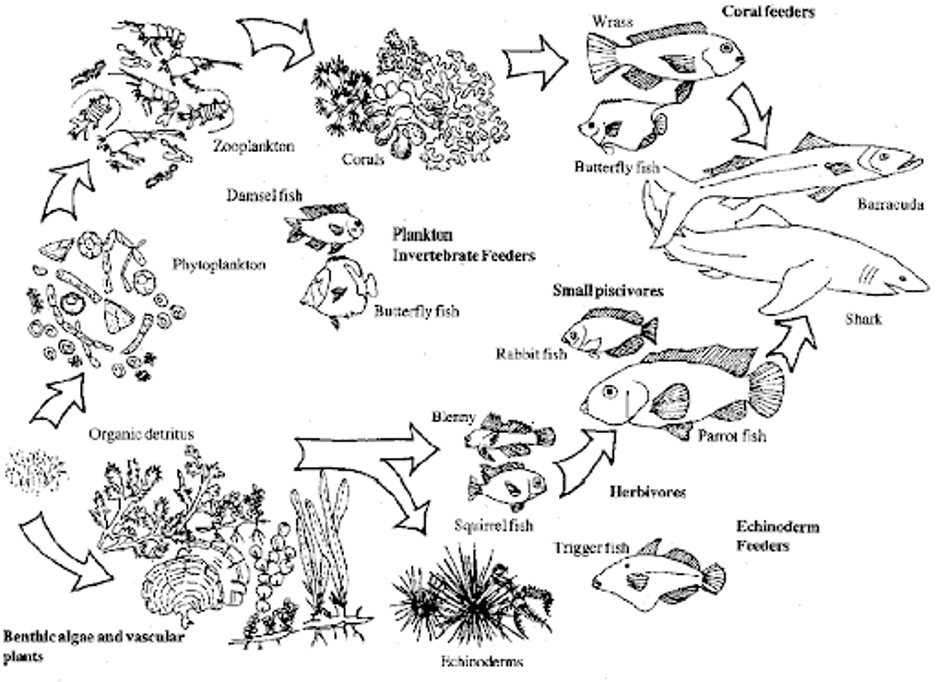
\includegraphics[width=\linewidth]{images/reeffoodweb}
\caption{The coral reef food web, or the relationship between successive trophic levels of the community, starts as any other food web, with energy being derived from the sun by primary producers via photosynthesis. These primary producers include seaweed, grass, phytoplankton, and perhaps most importantly, the zooxanthellae coral symbiotes. This is the largest group, as only about 10\% of the energy in each trophic level is passed to each successive level. The second trophic levels, the primary consumers, includes zooplankton, mollusks, squirrelfish, urchins, and of course, the coral polyps themselves. Following this are the secondary consumers, made up of triggerfish, Parrotfish, butterfly fish, and more. Finally, tertiary consumers like the reef shark and barracuda finish this food web, with detritivores like sea cucumbers or bacteria decomposing and recycling organic matter back into the ecosystem \citep{https://doi.org/10.1890/15-1492.1}. }
\label{fig:Example Reef Food Web}
\end{figure}

\begin{figure}
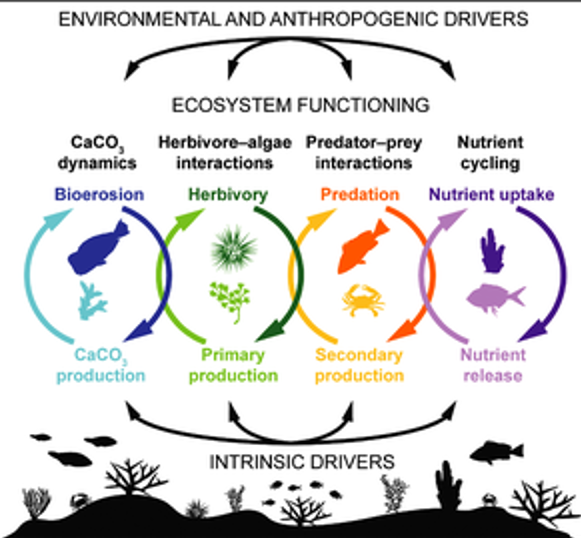
\includegraphics[width=\linewidth]{images/reefcycles}
\caption{The above cycles and reciprocal processes are vital for coral growth and survival. The first, blue cycle, calcium carbonate dynamics, is directly correlated with the coral skeleton formation. Bioerosion, or the breakdown of hard oceanic substrates, leaves behind calcium and carbonate ions, which coral polyps use to produce their limestone skeletons. The second, green cycle, herbivore-algae interactions, involves both primary production and herbivory. Photosynthetic organisms transform sunlight into chemical energy, which is then moved up in trophic levels by herbivores. A balance between the two must be maintained to prevent explosive growth of lower trophic levels, which in turn could suppress crucial processes carried out by other organisms in the ecosystem. Predator-prey interactions, the orange cycle, also regulate explosive trophic level growth, as successive trophic level limits the prior. Again, the balance keeps the biomass of one species from dominating and smothering other species. The final process driving success within the coral reef ecosystem is the purple cycle, nutrient cycling, or the uptake and release of nutrients among the organisms of the ecosystem. Nutrients must be moved efficiently and effectively in cycles, with a balance maintained between retention and reintegration \citep{https://doi.org/10.1002/fee.2088}. Figure from: \citep{https://doi.org/10.1002/fee.2088}. } 
\label{fig:Reef Ecosystem Functioning and Intrisnsic Drivers}
\end{figure}

\begin{figure}
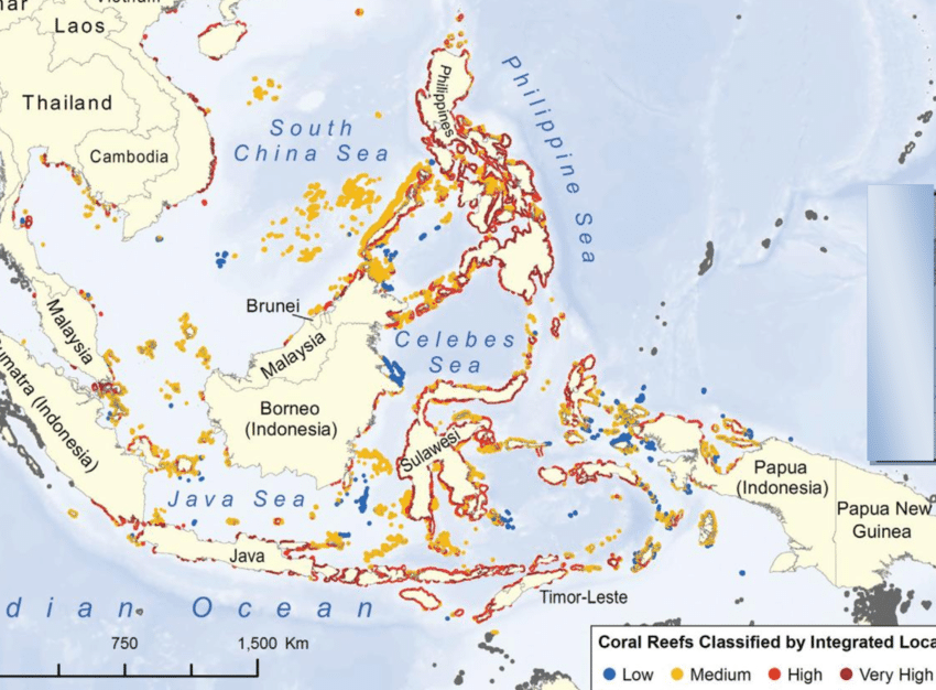
\includegraphics[width=\linewidth]{images/reefmap}
\caption{Coral reef locations are relatively limited, as the previously mentioned conditions must be satisfied, yet they can be found in over 100 countries, mainly between the Tropics of Cancer and Capricorn. As seen above on the map, reefs are concentrated in shallow waters surrounding many islands of the Indo-Pacific. Reefs surrounding both Indonesia and the Philippines compose a majority of not only Southeast Asian reefs, but also reefs worldwide.   Coral reefs cover 284,300 square kilometers (110,000 square miles) worldwide, yet the overall area of healthy reef is decreasing rapidly \citep{Watlas}.}
\label{fig:Map of Southeast Asian Coral Reefs}
\end{figure}

\begin{table}[h]
\caption{Southeast Asian Coral Reef Size by Country}
\subcaption{:Listed are some notable Southeast Asian countries and their respective reef areas. While Indonesia and the Philippines dominate total reef area, many coastal Southeast Asian countries have reefs of their own, all which face similar anthropologic pressures. Southeast Asia accounts for over a quarter of all the worlds coral reefs \citep{Watlas}.}
\label{tab:Southeast Asian Coral Reef Size by Country}
\begin{tabular}{llll}
Country     & World Reef Area Ranking & Reef Area (sq km) & Percentage of World Total Reef Area (\%) \\ 
\hline\hline
Indonesia   & 1                       & 51,020            & 17.95\% \\ 
\hline
Philippines & 3                       & 25,060            & 8.81\%  \\ 
\hline
Malaysia    & 17                      & 3,600             & 1.27\%  \\ 
\hline
Japan       & 23                      & 2,900             & 1.02\%  \\ 
\hline
Thailand    & 26                      & 2,130             & 0.75\%  \\ 
\hline
Myanmar     & 27                      & 1,870             & 0.66\%  \\
\end{tabular}
\end{table}

\begin{figure}
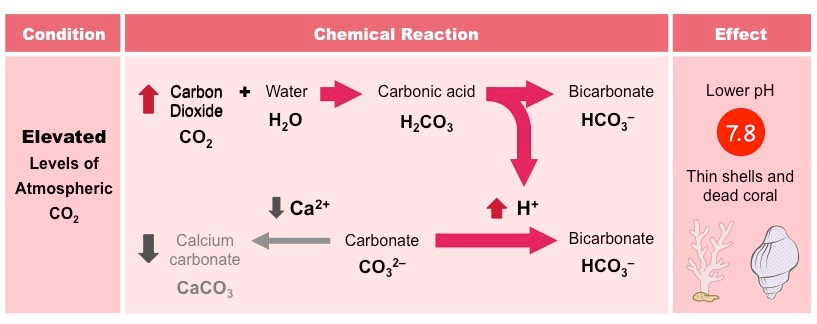
\includegraphics[width=\linewidth]{images/acidification2_med}
\caption{The above figure outlines the chemical reactions which connect ocean acidification with limestone formation. As carbon dioxide dissociates in the water, it creates carbonic acid, or H$_2$CO$_3$. The protons of carbonic acid are easily dissociated by the more polar water molecule (H$_2$O), thus dissociating and combining to form bicarbonate, or HCO$_3$. The dissociated protons may also form bicarbonate by reacting with carbonate ions. This chemical reaction removes carbonate ions from the water, which corals need to construct their calcium carbonate skeletons.}
\label{fig:Ocean Acidifcation Chemical Reaction and Its Carbonate Relation}
\end{figure}

\begin{figure}
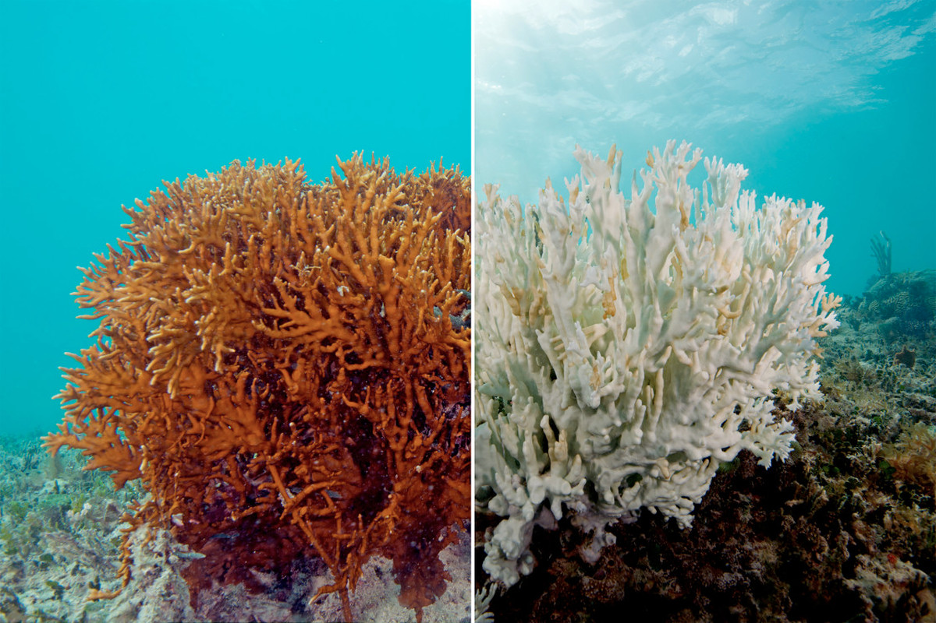
\includegraphics[width=\linewidth]{images/coralbleach}
\caption{This above split-image shows the same fire coral before (left) and after (right) coral bleaching has occurred. The vibrant colors on the left image result from the zooxanthellae symbiotes, and when the corals expel them, the ghostly white color seen on the right image is observed. This color change is universal across all coral species; only the color of the calcium carbonate skeleton remains after the algae are expelled.}
\label{fig:Coral Bleaching}
\end{figure}

\begin{figure}
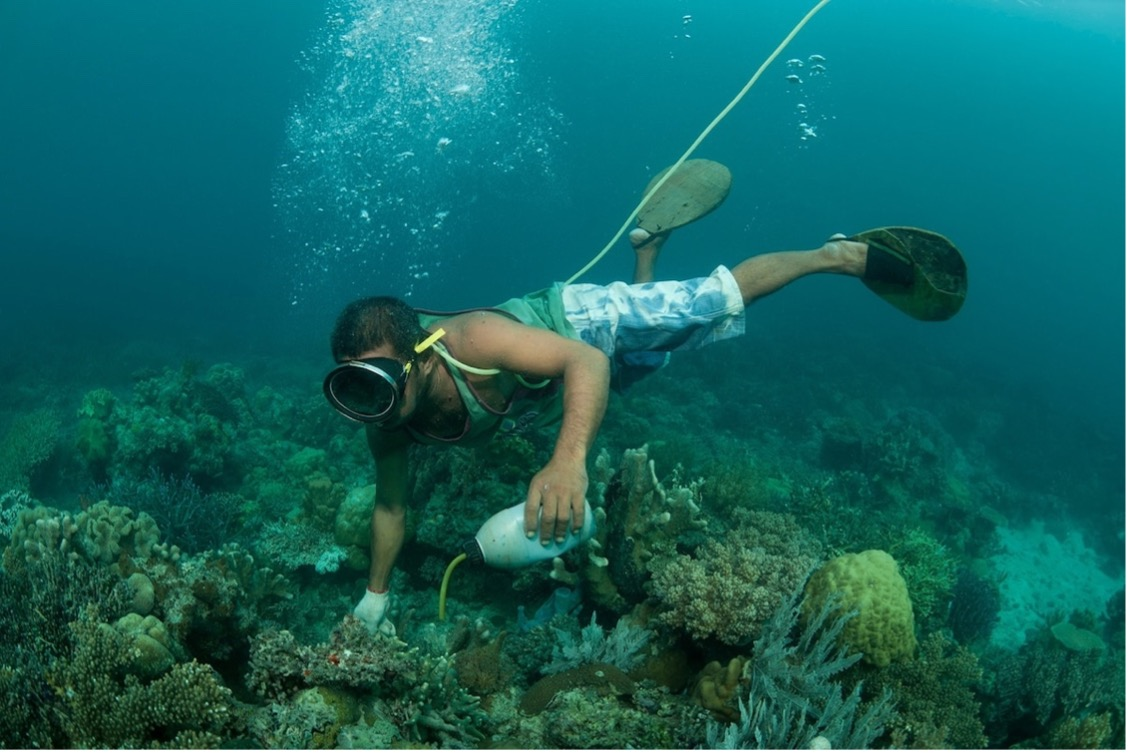
\includegraphics[width=\linewidth]{images/cyanidefishing}
\caption{:The diver in this picture is cyanide fishing in a Filipino reef. He uses cheap, makeshift gear which can be either made from scrap or repurposed. The warm, coastal waters allow him to dive without a wetsuit, only using wood planks nailed to slippers as fins. His bottle contains crushed sodium cyanide tablets dissolved in water, a lethal solution which will decimate the reef he is injecting it into.}
\label{fig:Cyanide Fishing}
\end{figure}

\begin{figure}
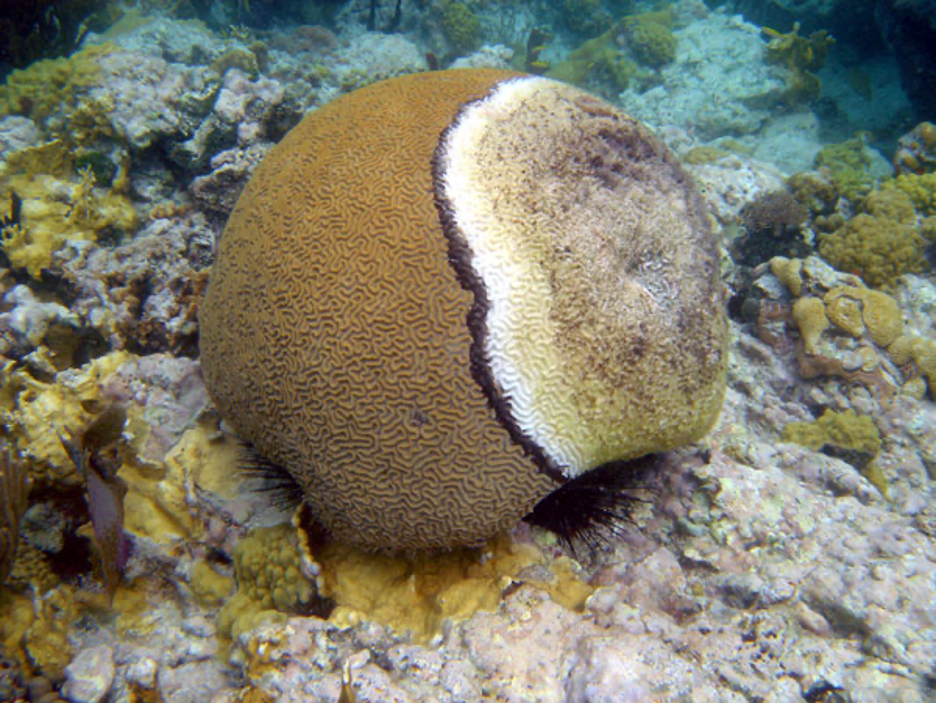
\includegraphics[width=\linewidth]{images/coraldisease}
\caption{:This picture shows a brain coral that has been infected with black-band disease. The left side of the coral is how healthy coral appears; the right side is diseased. This particular coral disease’s name is derived from the black circumferential band in the middle of the coral. As the disease progresses, the band travels along the coral, killing polyps and leaving behind a dying, empty skeleton (seen on the right half of the coral).}
\label{fig:Black Band Disease}
\end{figure}

\begin{figure}
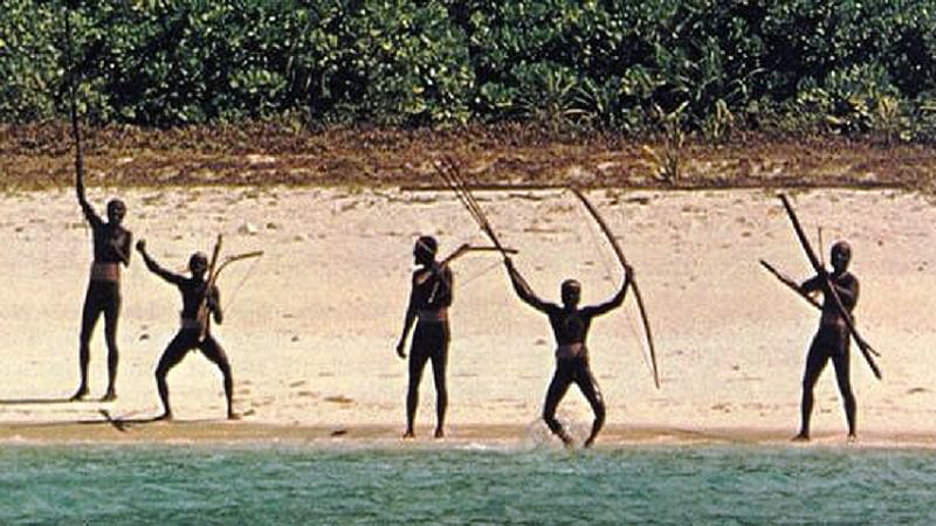
\includegraphics[width=\linewidth]{images/sentpeeps}
\caption{:The Sentinelese people are pictured above. When this picture was taken, they approached the bank and began making threatening advances towards the camera’s direction. The man on the far left throws a spear while the man on the far right readies an arrow. This hostility towards outsiders has allowed to Sentinelese to remain one of the last untouched indigenous groups in the world.}
\label{fig:An Interaction with The Sentinelese People }
\end{figure}

\begin{figure}
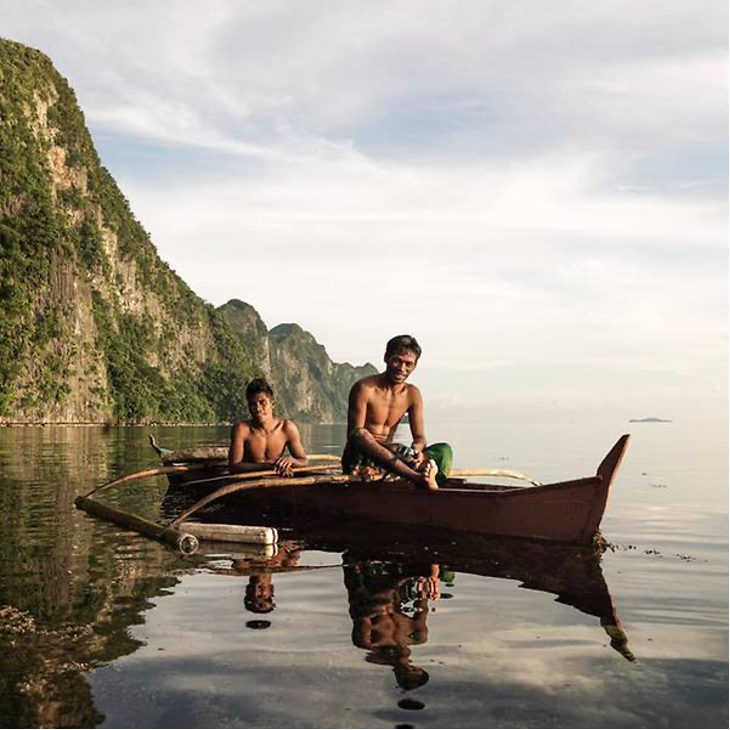
\includegraphics[width=\linewidth]{images/tagfish}
\caption{:The 12-15 million indigenous people living in the Philippines make up between 10-15\% of the population. 110 groups are officially recognized, yet there are many more who have not been officially recognized by the Philippines’ government \citep{4826000120100501}. Above pictured are the Tagbanua, one of these indigenous people groups of the Philippines. They either spearfish or fish from simple wooden boats like seen above. These boats are used to traverse the shallow reefs and harvest fish, lobster, squid, octopus, and other protein sources. Many other indigenous groups maintain a similar reef-relationship, one consisting of simple fishing practices, and transportation methods \citep{4826000120100501}.}
\label{fig:Tagbanua Fishing}
\end{figure}

\begin{figure}
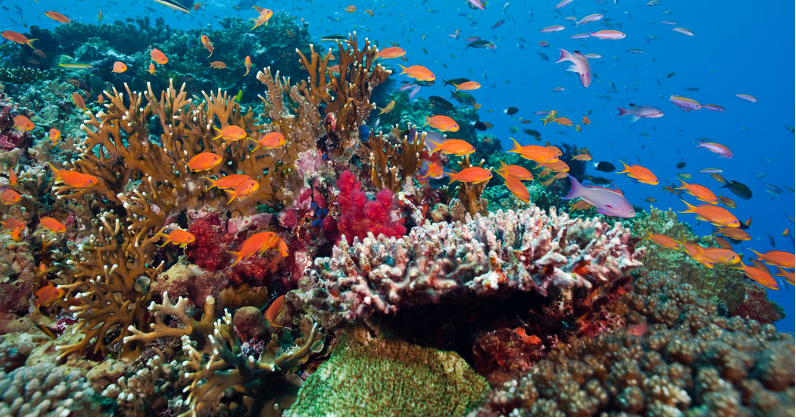
\includegraphics[width=\linewidth]{images/reefbigchillin}
\caption{:Pictured is a healthy Southeast Asian coral reef. Bursting with color and biodiversity, reefs like these support lives for thousands of species, including humans. Reef restoration and protection are crucial to maintaining already thriving reefs like this and also reviving the many degraded reefs of Southeast Asia. Reef conservation will allow these coral reefs to remain rich in biodiversity and continue sustaining the indigenous peoples and coastal communities of Southeast Asia.}
\label{fig:A Healthy Southeast Asian Coral Reef}
\end{figure}


\chapter{Nuclear Power and Nuclear Waste}

\section{Current and Future Energy Needs}



\chapter{Air Pollution \& Social Justice in Hong Kong}

\chapterauthor{Neenah Vittum}

\section{Science of Air Pollution}

\subsection{Overview of the layers of the atmosphere/atmospheric gases}

What part of the atmosphere does air pollution affect?

What is air pollution?

Overview of different types of air pollution

\section{Major Sources → Use as geographical overview}

\subsection{General common sources of air pollution all over the world}

\subsection{East Asian countries/communities and their prominent air pollution sources}

Shipping

Traffic Emissions

Commercial and otherwise

Coal

Urban Development

Manufacturing

Other

The transboundary issue and its implications in regulation and politics

Impacts

Human health

Environmental Health

Greenhouse gas emissions and global warming

Both

Visibility

Environmental Justice

Case Study: Hong Kong

The Intersection of Air Pollution and Other Environmental Issues

Many environmental issues are interconnected

Air pollution and deforestation

Air pollution and urbanization/industrialization

Other Issues (To Explore)

Goals/Other Ideas/Questions

Ground information in geography and relevant examples

Incorporate stories and person accounts

slow violence → environmental justice issues

Maybe activist or someone who has suffered the issues firsthand

Draw people into the empathy

Use stories and descriptions to describe places

What is the best way to section the chapter?


\chapter{Flood Pulse System in East Asia}

\chapterauthor{Kristin Gabriel}

\section{Introduction}

What is the flood pulse system?

Seasonality

Ecosystem Services

Fish stocks

Flooded forests

How the flood pulse system influences the Tonle Sap Ecosystem

Timing of Flood Pulse

Magnitude of Flood Pulse

Duration of Flood Pulse

Influence of flood pulse system on people and their livelihoods

Fisheries

Immigration and emigration

Human Impacts on the flood pulse system

Climate change

Dam development

Case Study: Cambodia and the Tonle Sap


\chapter{Hydroelectric Dams in East Asia}

\section{Introduction}

Basic facts about dams in East Asia


Statistics on how many, size, scale, location etc.

Function of the Dam 

How it generates electricity/how much

Different types of dams (multi/single use etc.) 

Immediate ecological impacts 

Positive: 

Flood control, electricity generation, improved water quality 

Negative: 

Decreased water quality, flooding, sedimentation, habitat loss, deforestation, salinization etc... *note: the ecological impacts may be too many to go completely in depth into so perhaps a paragraph or subsection of each as opposed to a 7 page explanation of each 

Anthropological impacts 

Supposedly positive (I.e. employment etc...)

Negative: displacement, loss of cultural sites, diseases 

Displacement

Policy/government action/regulation  (policies that exist or propose solutions)

\section{Conclusion}



\chapter{Climate Change and Food Security in Myanmar}



\section{Climate Change, Climate Change Response in Myanmar}


General history of rice production and food demand in Myanmar. 

Impact on credit policy on rice 

Impact of infrastructure development on rice production

Study of the constraints of rice production in Myanmar

The effect of a command economy on food production in Myanmar 

Overall review on demand for food in Myanmar 

Possible implementation of SRI (systemic rice intensification) in order to increase rice yields in Myanmar

Transition from talking about rice production

sea-level rise

subsidence

coastal erosion

coastal flooding

Impact of climate change on rice production in Southeast Asia

Monsoon Season effect on Ayeyarwady River Badin

Sea Level Rise 

Sea level rise effect on global markets/rice production


Subsidence

Subsidence in Yangon, Myanmar

interview segments/personal experiences of rice farmers


Roles of the Burmese government

\section{Conclusion}

Reminders/Areas of Focus




\chapter{Disasters, Typhoons and Phillipines}

\chapterauthor{Ian Horsburgh}

\section{What are Typhoons?}



\chapter{Climate Infrastructure in Vietnam}

\section{Introductory}

How climate change will impact Vietnam

Flooding (especially coastal urban areas)

Sea Level Rise

Land Erosion

Health outcomes

Current Adaptation Plans

Strengthen existing barriers and infrastructure

Adapt cities expecting sea level rise

Withdraw from the coastlines in areas that are well below sea level

What's Needed for the Future

Stronger healthcare system

Support for farmers and agricultural workers

Support for rural population near Mekong and Red river deltas

\section{Conclusion}

Implications for other places in the region


\chapter{Waste Management for a Circular Economy}

\section{Life-Cycle}

\subsection{Collection}

\subsection{Transport}

Treatment

Disposal

Sectors:

Industrial

Household

Biological 

Types of Waste:

Solid:

Liquid

Gaseous waste

\section{Biomimicry}

\subsection{Circularity}

Examples in Nature

Education:

Teach people to be mindful and live sustainably

Social PsychologyProblems and New Approaches: 

Sustainability

Incineration \& Dumping

Recycle \& Reuse

Resource Recovery


\chapter{Plastic and Packaging in Japan}

\section{Introductiona and Goals?}

Plan: Use Japan's unique plastic packaging as a lens to view plastic waste management. I can bring in benefits of their plastic use, like cultural significance of beautiful wrapping and food safety, and then discuss plastic pollution as a larger issue in East Asia, bringing in examples of blame placing, and of course discussing potential solutions on both international and local scales. 

\section{Plastic Pollution and Waste Management in East Asia} 

\subsection{Statistics/comparisons}

graphs and images will help with perspective

\subsection{History of plastic waste issues in East Asia}

\subsubsection{Are specific companies/industries responsible responsible}

what kinds of plastic waste are there (sector break down)? 

\subsubsection{Where in the world did the ubiquitous usage of single use plastics come from?}

General blame placing/biases/rhetorical 

examples of discourse around plastic waste in East Asia. Why does any of this matter(needs its own section)?

Plastic waste trade? 

\url{https://link.springer.com/article/10.1007%2Fs10163-004-0115-0}

\url{https://www.sciencedirect.com/science/article/abs/pii/S0956053X20305602}

Blame placing through both rhetoric and scientific studies

(this source is a very data based study that concluded that the vast majority of plastic pollution comes from a few sources in Asia/Africa... I want to explore what they might not have taken into account when collecting data)

\url{https://science.sciencemag.org/content/347/6223/768}

\url{https://pubs.acs.org/doi/10.1021/acs.est.7b02368}

\url{https://www.dw.com/en/whose-fault-is-plastic-waste-in-the-ocean/a-49745660} (found the two above studies through this article)

Japan Specific (I need to break these into hierarchies of significance), some sections, the first  few will be more data based, the second half will be more rooted in sociological primary sources.

Waste management issue overview

Sector Break Down/ responsible parties in Japan

Impacts of plastic pollution on different groups within Japan

Cultural significance of wrapping

Food safety

Gov action/recycling/current efforts

Activism

Potential solutions moving forward rooted in current activist efforts/respect to culture

\url{https://www.pnas.org/content/117/33/19844.short}

\url{https://www.jstor.org/stable/432317?seq=1}

\url{https://onlinelibrary.wiley.com/doi/abs/10.1002/1099-1522(200003/04)13:2%3C45::AID-PTS496%3E3.0.CO;2-%23}






\backmatter

\part{Backmatter}

The back matter often includes one or more of an index, an afterword, acknowledgments, a bibliography, a colophon, or any other similar item. In the back matter, chapters do not produce a chapter number, but they are entered in the table of contents. If you are not using anything in the back matter, you can delete the back matter TeX field and everything that follows it.

\printglossary

\renewcommand\bibname{References}
\setlength{\bibsep}{2\baselineskip}
\setlength\bibindent{.5in}
\bibliographystyle{plainnat}
\bibliography{References}

\end{document}
